\documentclass[Integrationstest/Integrationstest_main.tex]{subfiles}
\begin{document}

\section{Integrationstest Playerside}\label{sec:integration_playerside}
\subsection{Introduktion}
Dette afsnit beskriver den integration og de tests mellem undermodulerne, der har lavet for PlayerSide-modulet. PlayerSide-modulet består henholdt systemarkitekturen af følgende hardware moduler:
\begin{itemize}
    \item 6 CupHolders, hver bestående af 
    \begin{itemize}
        \item CupSensor.
        \item CupLight.
    \end{itemize}
    \item CupHolderController
    \item PSoCPlayerSide.
\end{itemize}
Det er vigtigt, at lægge mærke til at hardware for CupSensor og CupLight allerede var "integreret" til et modul inden denne test, se modultest CupHolder. 

Følgende software moduler skulle også integreres til et samlet modul:
\begin{itemize}
    \item CupSensor\_IF.
    \item CupLight\_IF.
    \item GameController.
    \item RPi\_IF.
\end{itemize}


\subsection{Integrationstest mellem GameController og CupLight}
Det blev først besluttet at lave integrationen mellem GameController og CupLight, da det på denne måde var muligt at få visuelt feedback på sekvensen af GameController. Denne form for integration kan siges at være top-down.  Derudover var det også muligt at simulere states fra RPi gennem brug af WaveForms Protocol funktionen. 
\subsubsection{Testopstilling}
Til integrationstesten blev der anvendt CupHolder prototypen set på figur \ref{fig:Cupholder_integration}
\begin{figure}[H]
    \centering
    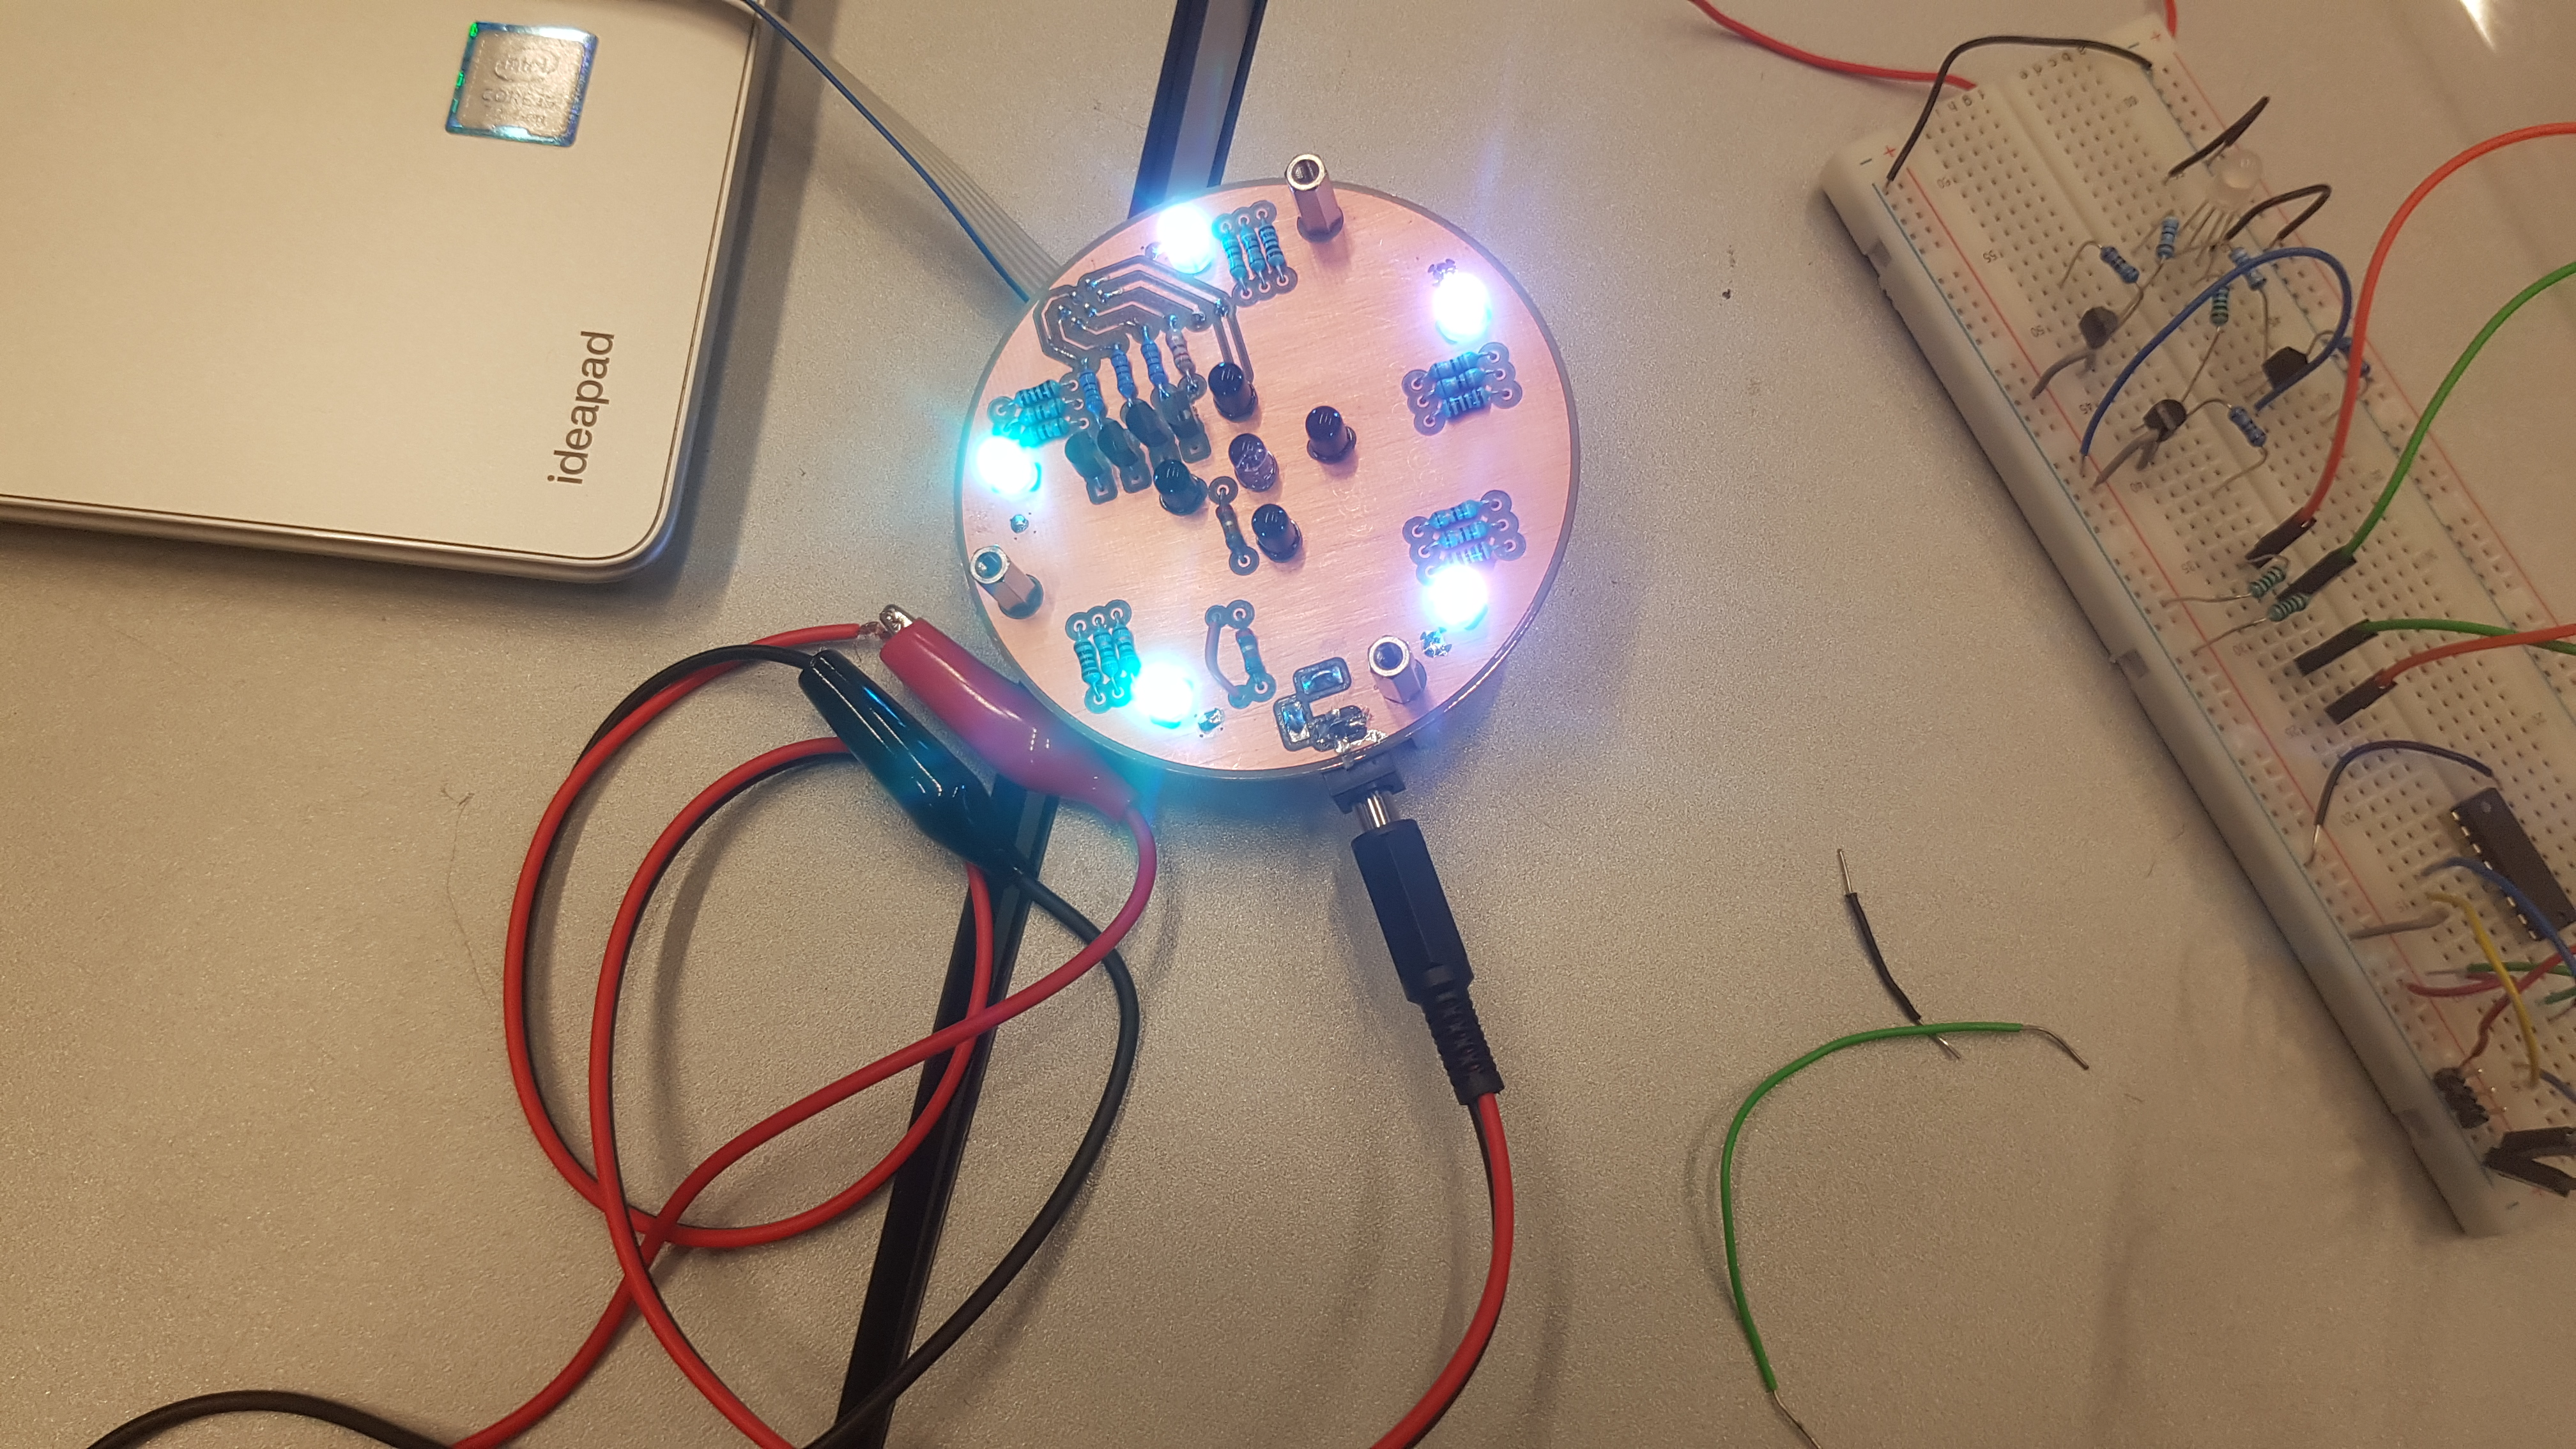
\includegraphics[width=\textwidth]{Integrationstest/Integrationstest_PlayerSide/graphics/CupHolder.jpg}
    \caption{CupHolder i integrationstest}
    \label{fig:Cupholder_integration}
\end{figure}

Derudover blev der anvendt den tilhørende hardware controller til lyset se figur \ref{fig:CupLightCtrl_integration}.

\begin{figure}[H]
    \centering
    \includegraphics[width=\textwidth]{Integrationstest/Integrationstest_PlayerSide/graphics/LightController.jpg}
    \caption{CupLightController i integrationstest}
    \label{fig:CupLightCtrl_integration}
\end{figure}

Der blev også anvendt AnalogDiscovery til at sende beskeder, der stemmer overens med den angivende protokol se \ref{fig:Protocol_integration}.
\begin{figure}[H]
    \centering
    \includegraphics[width=\textwidth]{Integrationstest/Integrationstest_PlayerSide/graphics/Protocol.jpg}
    \caption{CupLightController i integrationstest}
    \label{fig:Protocol_integration}
\end{figure}
\subsubsection{Fremgangsmetoden for test}
Denne test blev foretaget ved at gennemløbe de forskellige states i GameController, hvor states blev kontrolleret af de I2C beskeder, der blev sendt fra AnalogDiscovery. Det blev først testet, hvorvidt states opdaterede lyset i forbindelse med de forskellige states,\textit{Starting}, \textit{won} og et \textit{Loss}. Hertil blev der brugt default farver \lstinline|missingCupColor={255,0,0}|(Rød), \lstinline|placedCupColor={0,0,255}|(Blå), \lstinline|myColor={255,0,255}|(Lilla) og \lstinline|opponentColor={0,255,255}|(Cyan). Herefter blev det testet, hvis der kom et signal fra CupSensor om at en bold var ramt i ved at sende en kode, der stemte overens med protokollen for denne. 

\subsubsection{Resultater}
Testresultaterne viste at ved at stubbe forskellige sensor og I2C inputs, så resulterede det i de forventede farve kombinationer, som forklaret i fremgangsmetoden. Disse farvekombinationer vises ikke  i dette afsnit, men kan ses i funktion med sensoren i næste afsnit.

\subsection{Integrationstest med CupSensor}
Næste skridt i integrationen var så at integrere kopsensoren med de to allerede integrerede moduler. 
\subsubsection{Testopstilling}
Til integrationstesten blev der anvendt en samlet testopstilling, hvor de tidligere nævnte dele gik igen, sammen med et filter til sensoren.

\subsubsection{Fremgangsmetoden for test}
Igen blev testene foretaget, ved states blev kontrolleret af de I2C beskeder, der blev sendt fra AnalogDiscovery. Denne gang kunne states testes,\textit{Starting}, \textit{won} og et \textit{Loss} testes fuldt ud for PSoC idet sensoren kunne give inputs. Til denne test blev der igen anvendt default farver \lstinline|missingCupColor={255,0,0}|(Rød), \lstinline|placedCupColor={0,0,255}|(Blå), \lstinline|myColor={255,0,255}|(Lilla) og \lstinline|opponentColor={0,255,255}|(Cyan). 

\subsubsection{Resultater}
Først blev det testet, hvor programmet startede op i \textit{Idle}. Dette ses af figur \ref{fig:int_playerside_idle}.
\begin{figure}[H]
    \centering
    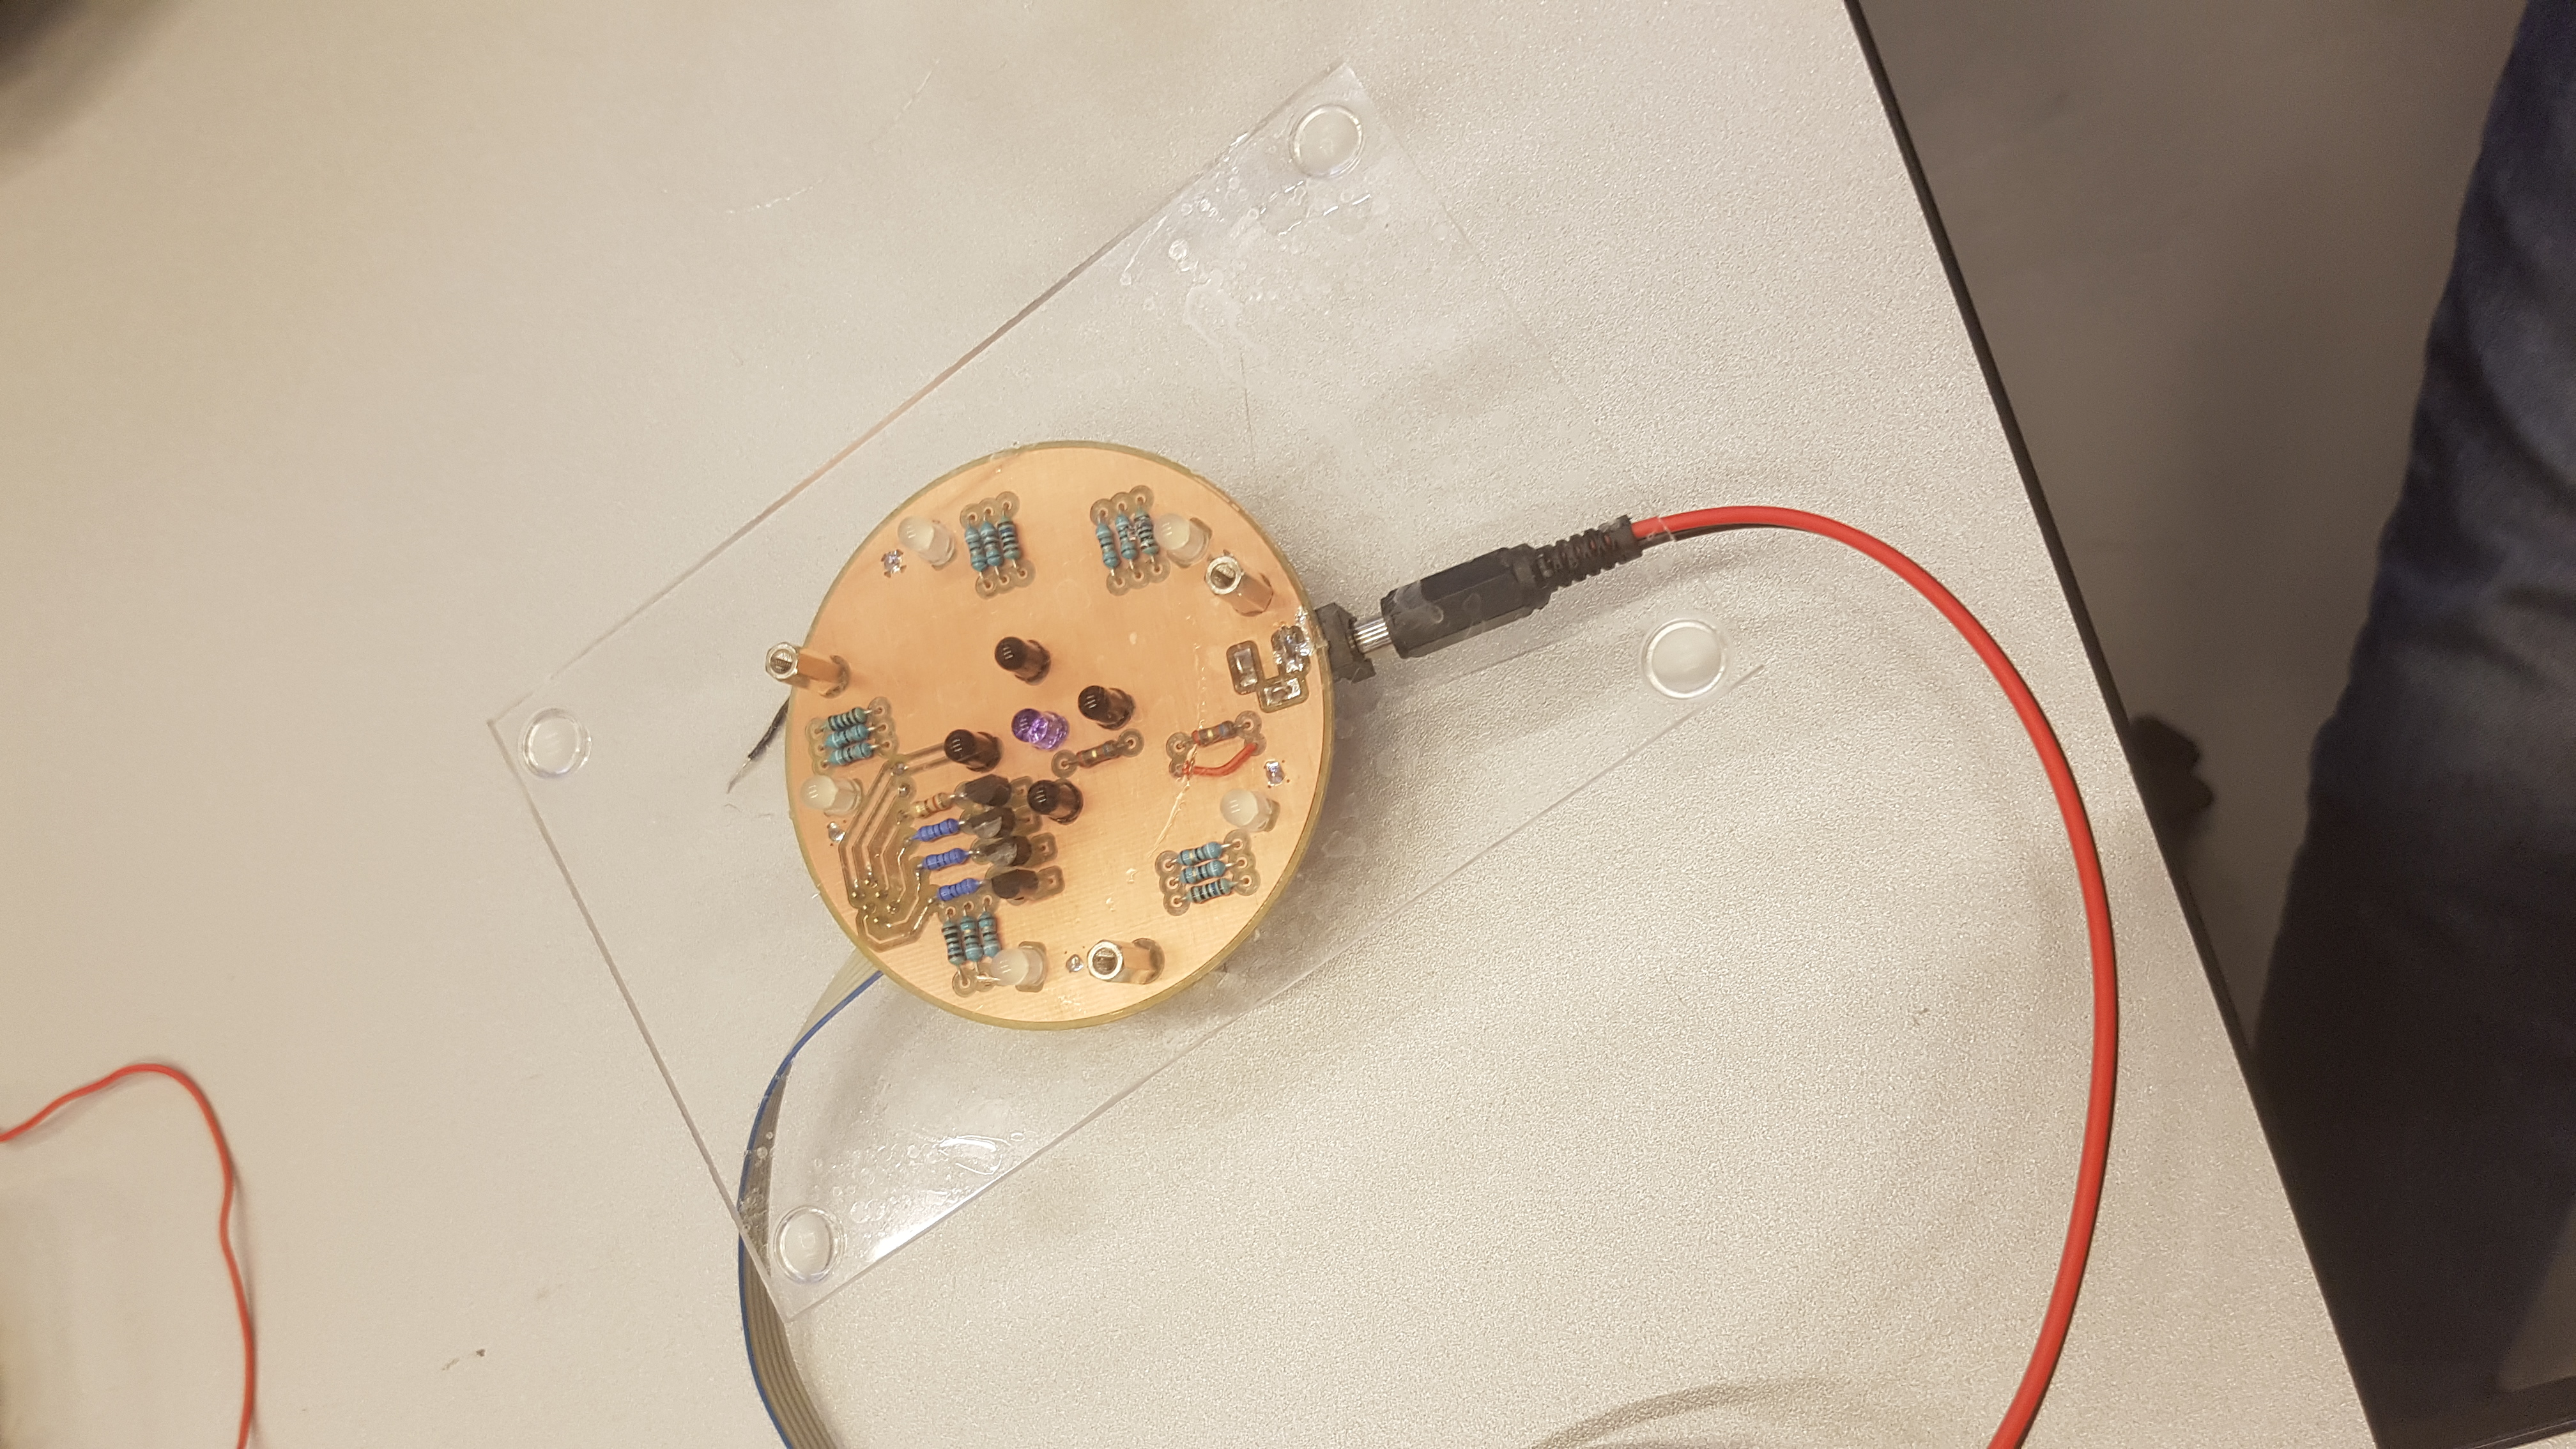
\includegraphics[width=\textwidth]{Integrationstest/Integrationstest_PlayerSide/graphics/CupSensorInt/IDLE.jpg}
    \caption{PSoC playerside ved state IDLE}
    \label{fig:int_playerside_idle}
\end{figure}

Herefter sendes en kommando med AnalogDiscovery for at skifte state til \textit{Starting}, dette giver følgende på CupHolder i figur \ref{fig:int_playerside_starting_no_cup}.
\begin{figure}[H]
    \centering
    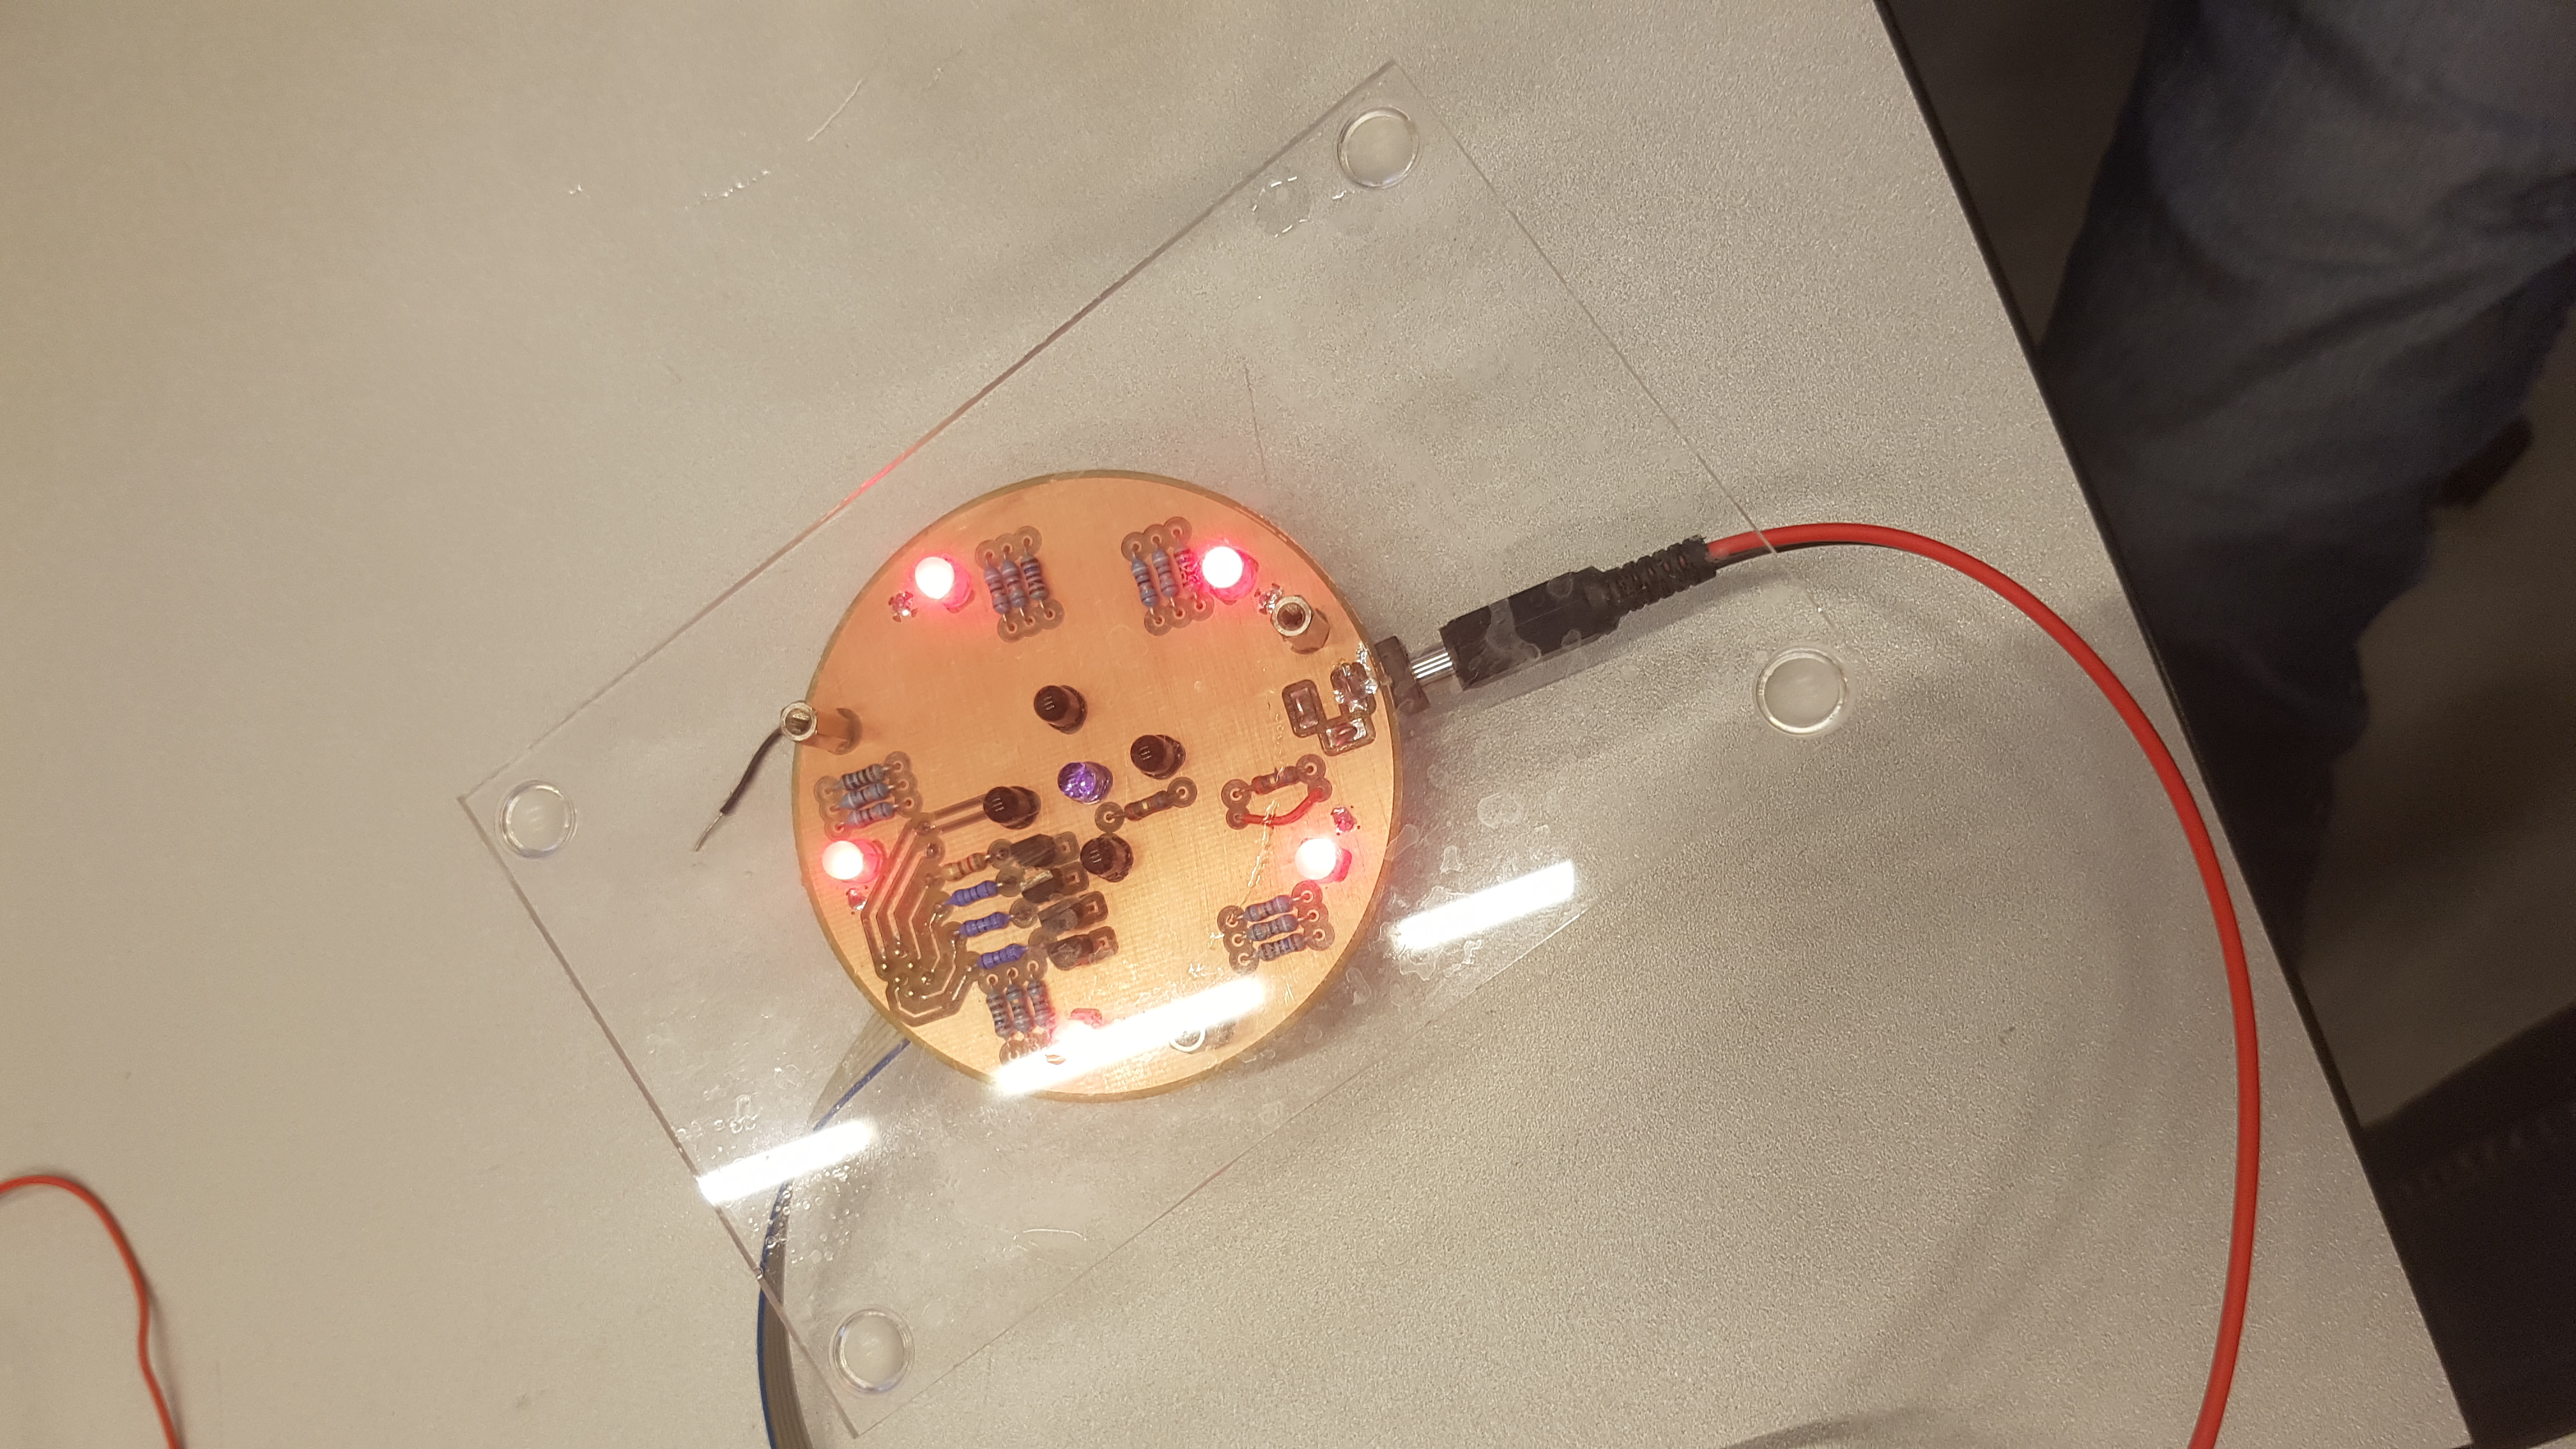
\includegraphics[width=\textwidth]{Integrationstest/Integrationstest_PlayerSide/graphics/CupSensorInt/STARTING_no_cup.jpg}
    \caption{PSoC playerside ved state STARTING og ingen kop}
    \label{fig:int_playerside_starting_no_cup}
\end{figure}

Der sættes så en kop på kopholderen, hvilket giver det følgende i figur \ref{fig:int_playerside_starting_cup}
\begin{figure}[H]
    \centering
    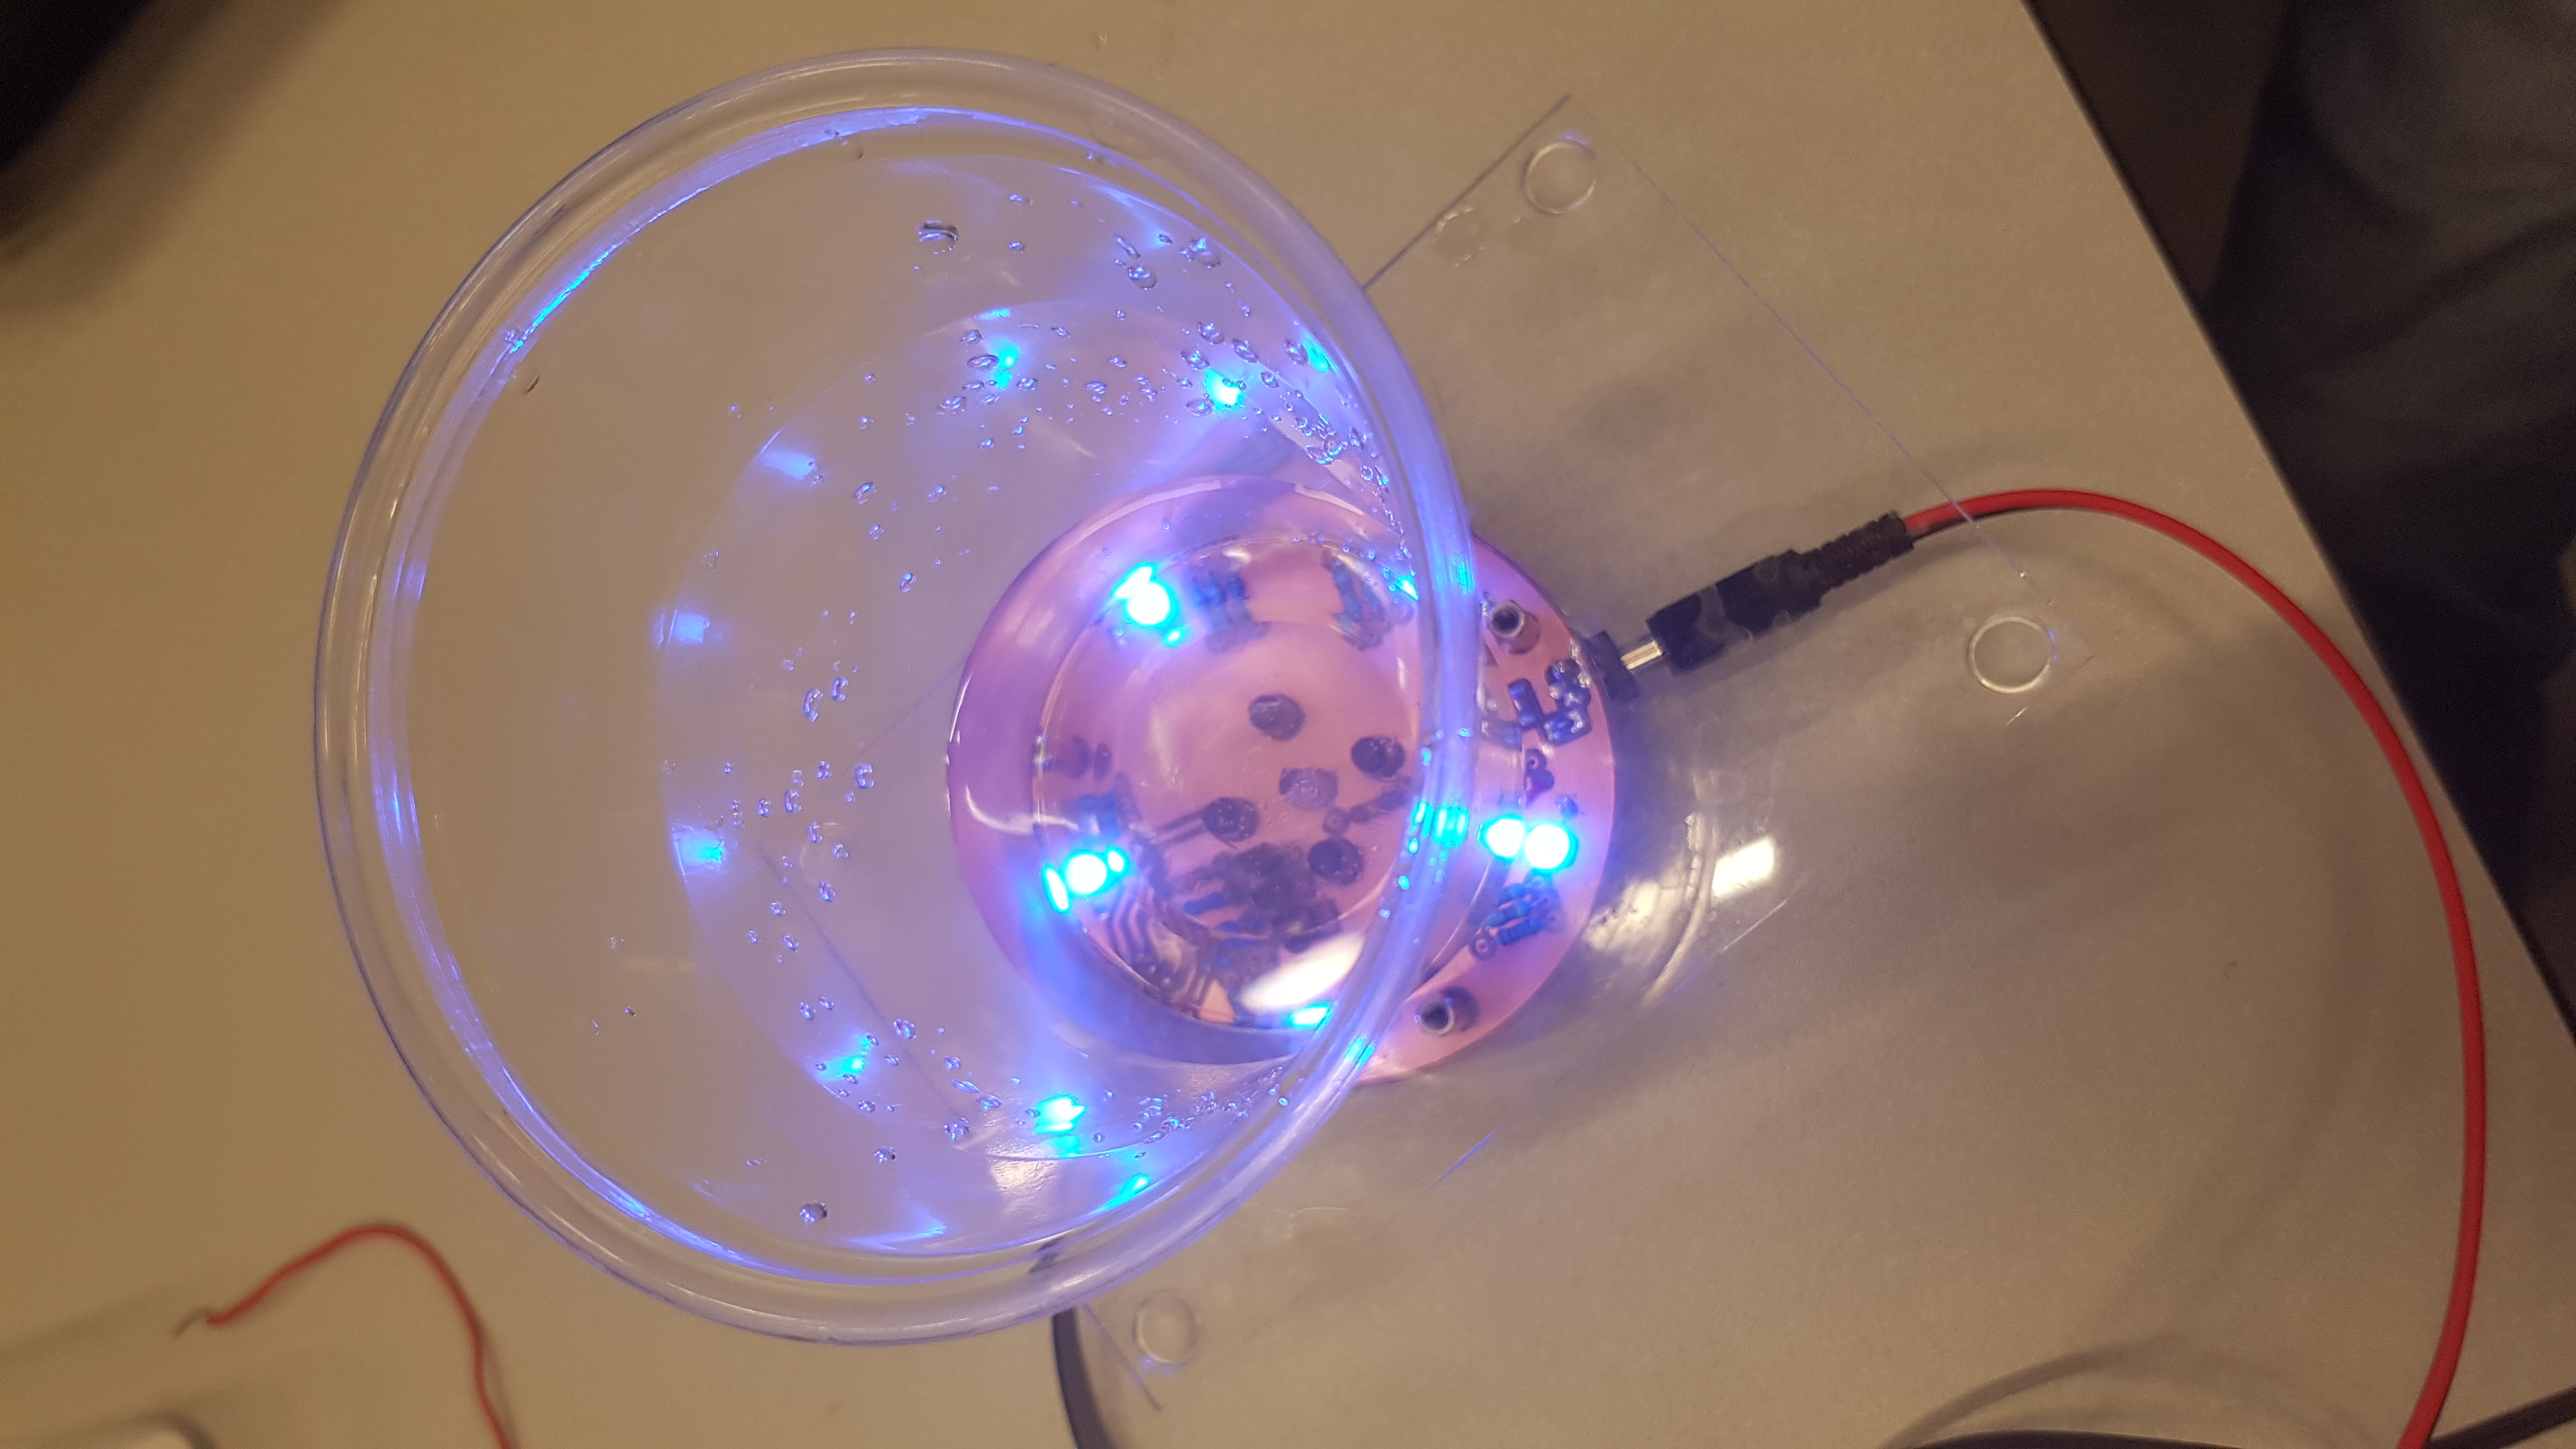
\includegraphics[width=\textwidth]{Integrationstest/Integrationstest_PlayerSide/graphics/CupSensorInt/STARTING_cup.jpg}
    \caption{PSoC playerside ved state STARTING, ved placering af kop}
    \label{fig:int_playerside_starting_cup}
\end{figure}

Der kastes så en bold i koppen for at teste, om den blinker, hvilket den ikke gør som det ses i figur \ref{fig:int_playerside_starting_no_blink}
\begin{figure}[H]
    \centering
    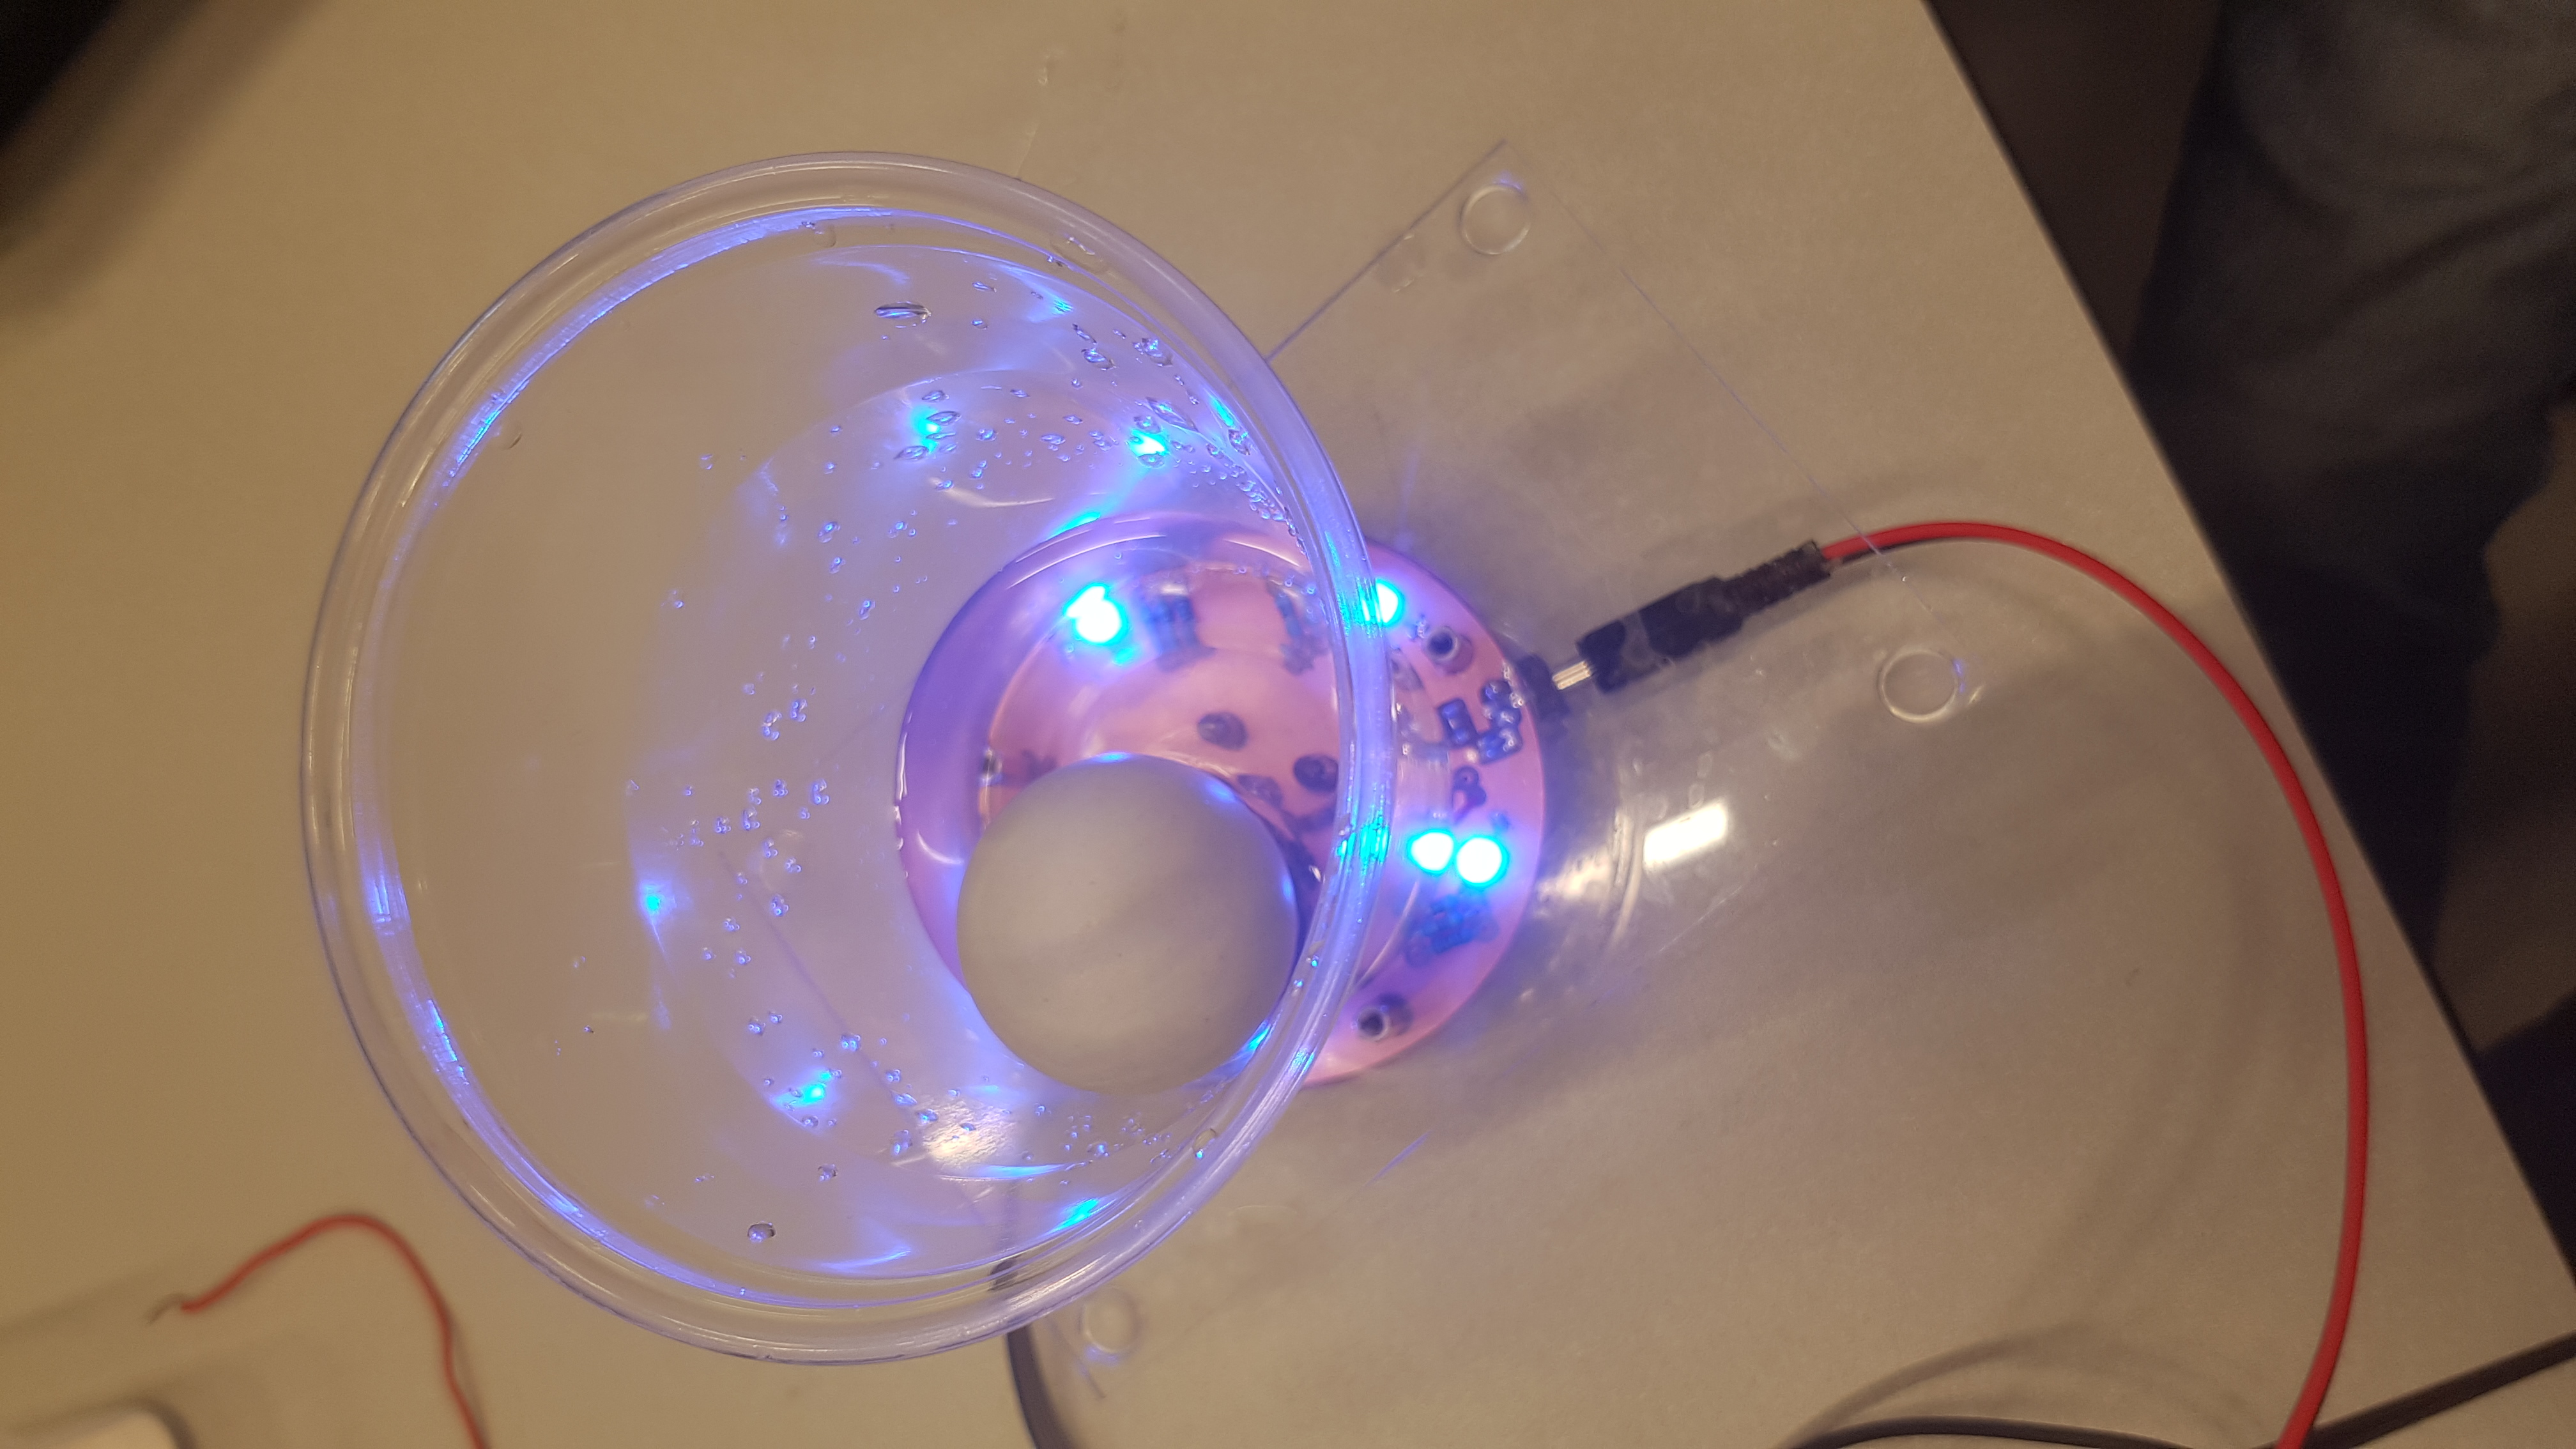
\includegraphics[width=\textwidth]{Integrationstest/Integrationstest_PlayerSide/graphics/CupSensorInt/STARTING_no_blink.jpg}
    \caption{PSoC playerside ved state STARTING, med bold i kop}
    \label{fig:int_playerside_starting_no_blink}
\end{figure}

Herefter skiftes state igen med AnalogDiscovery for at gå til state \textit{Playing}. Hvis der først testes uden nogen kop, så fås følgende i figur \ref{fig:int_playerside_playing_opp}.
\begin{figure}[H]
    \centering
    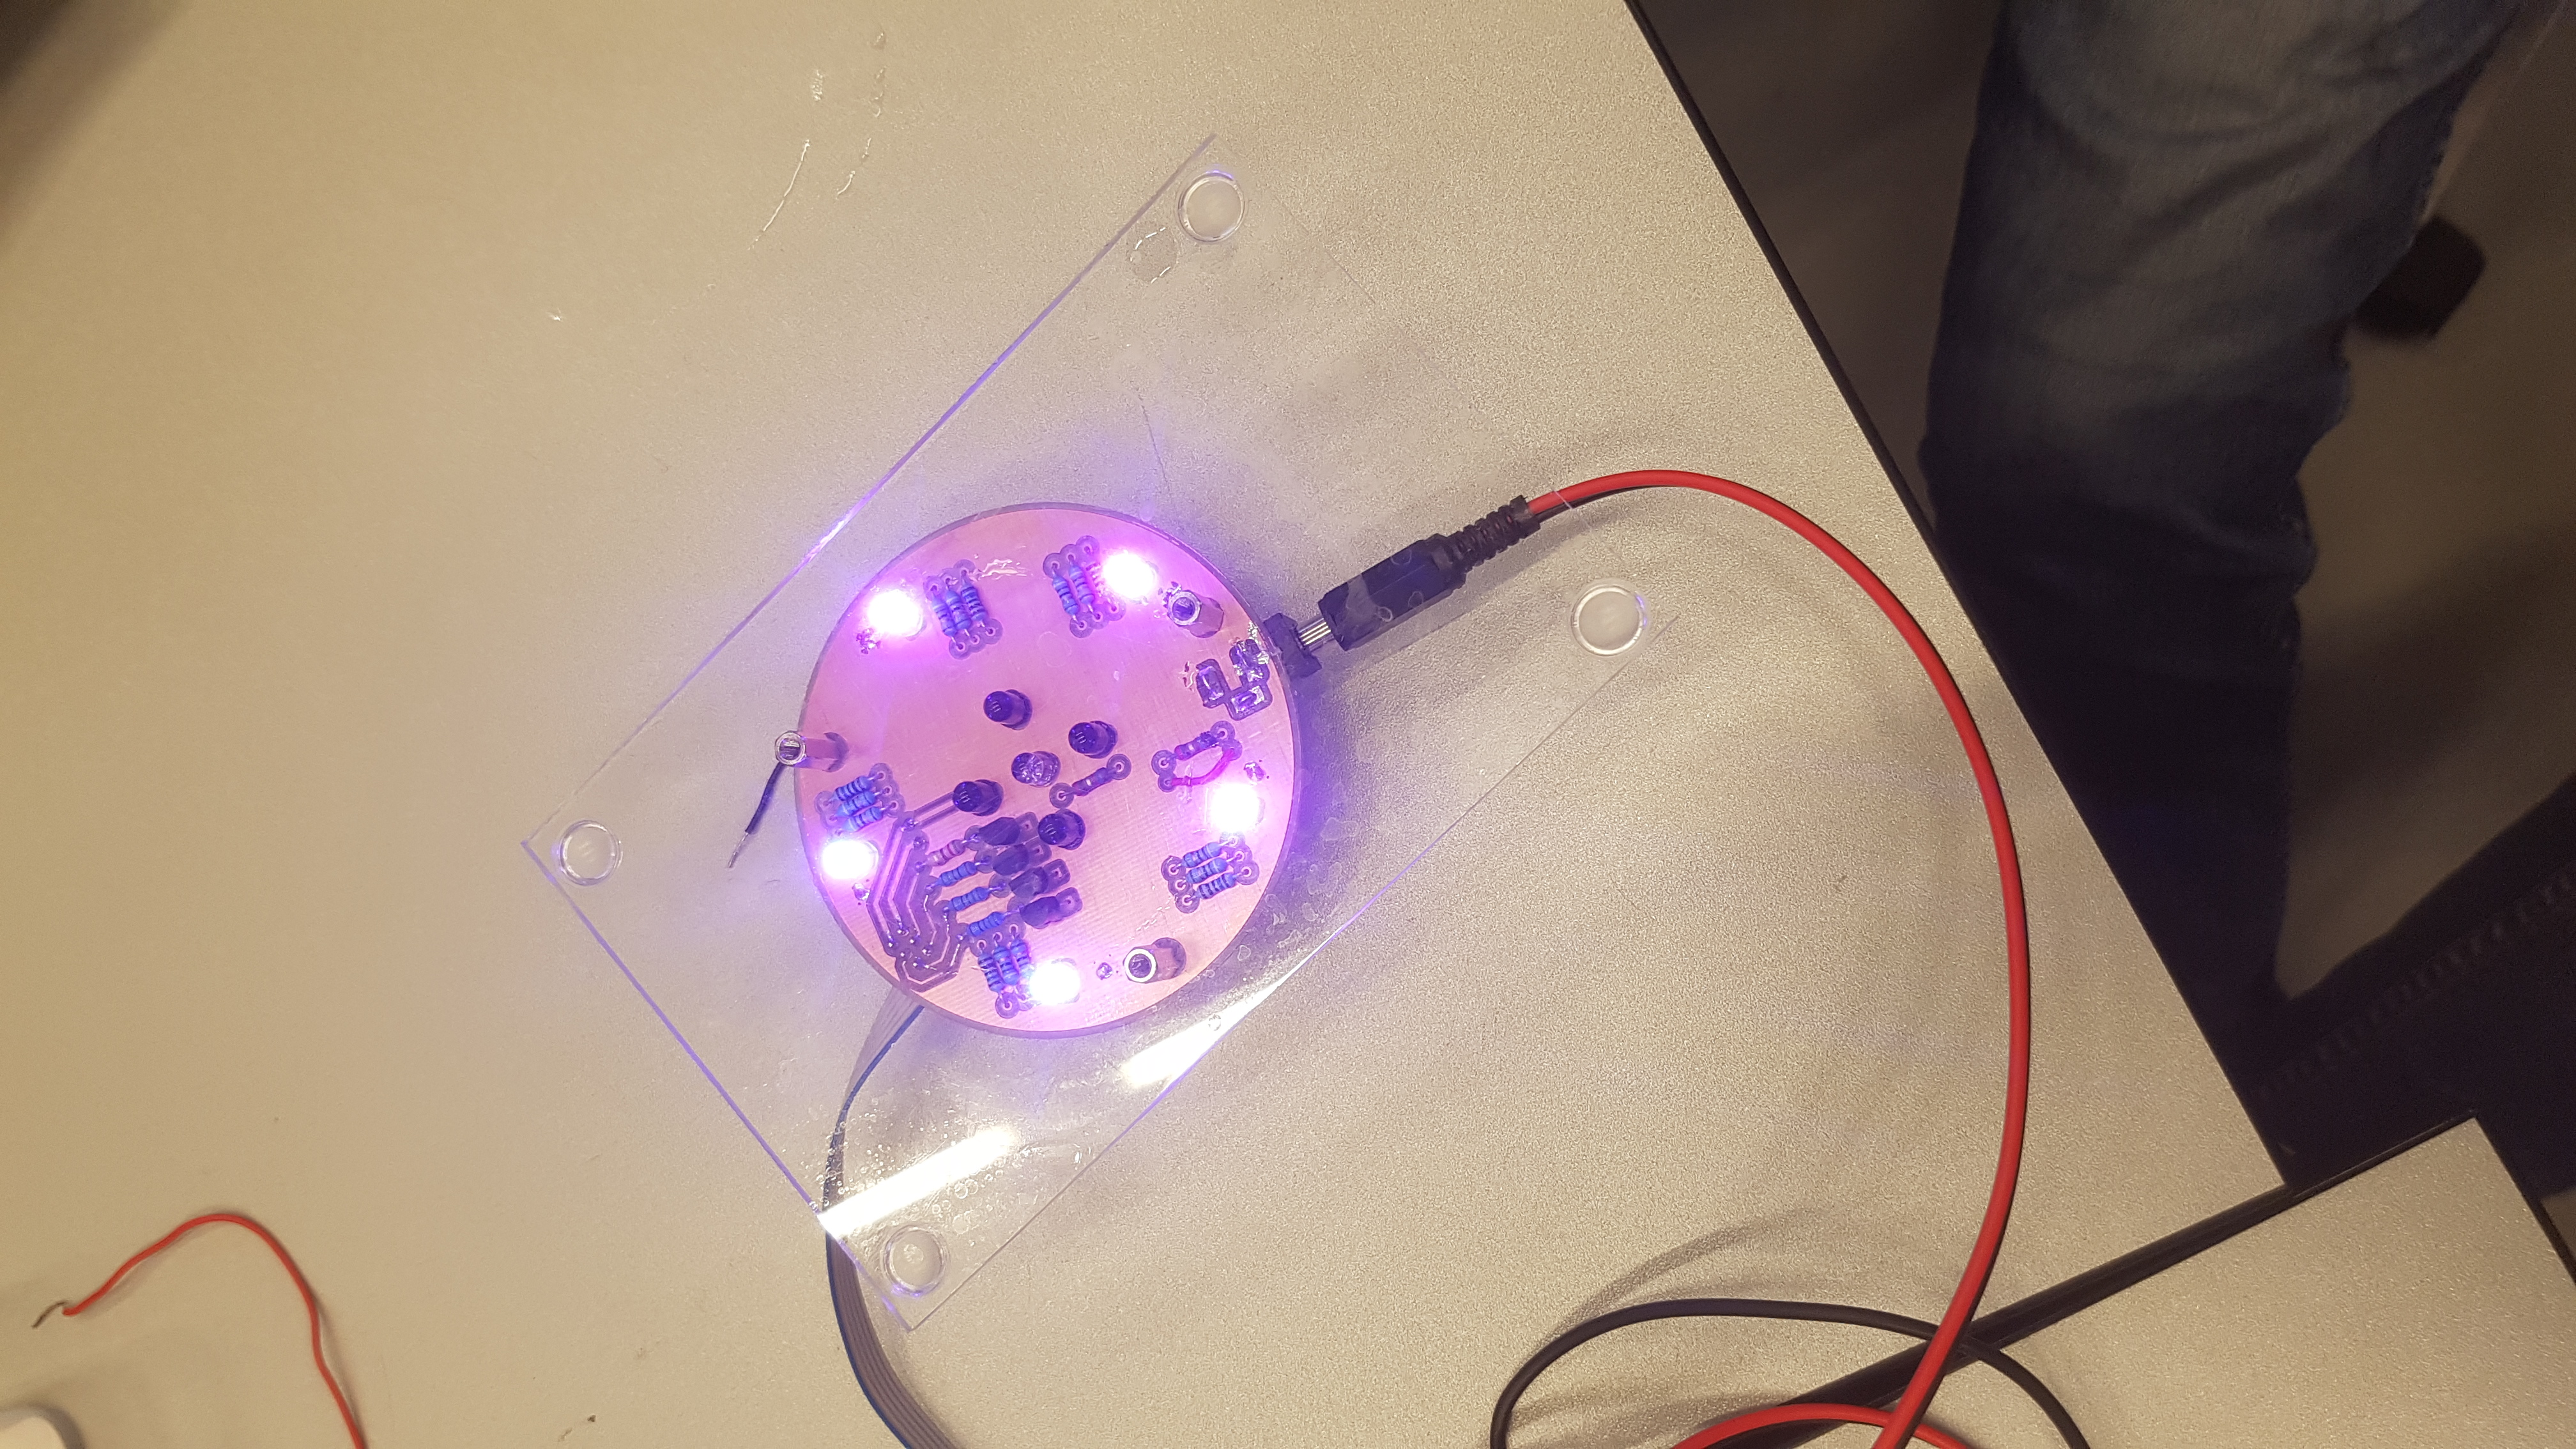
\includegraphics[width=\textwidth]{Integrationstest/Integrationstest_PlayerSide/graphics/CupSensorInt/PLAYING_opp_col.jpg}
    \caption{PSoC playerside ved state PLAYING uden kop}
    \label{fig:int_playerside_playing_opp}
\end{figure}

Herefter sættes en kop på kopholderen for at symbolisere en kop ikke er ramt endnu. Se figur \ref{fig:int_playerside_playing_my}.
\ref{fig:int_playerside_playing_opp}.
\begin{figure}[H]
    \centering
    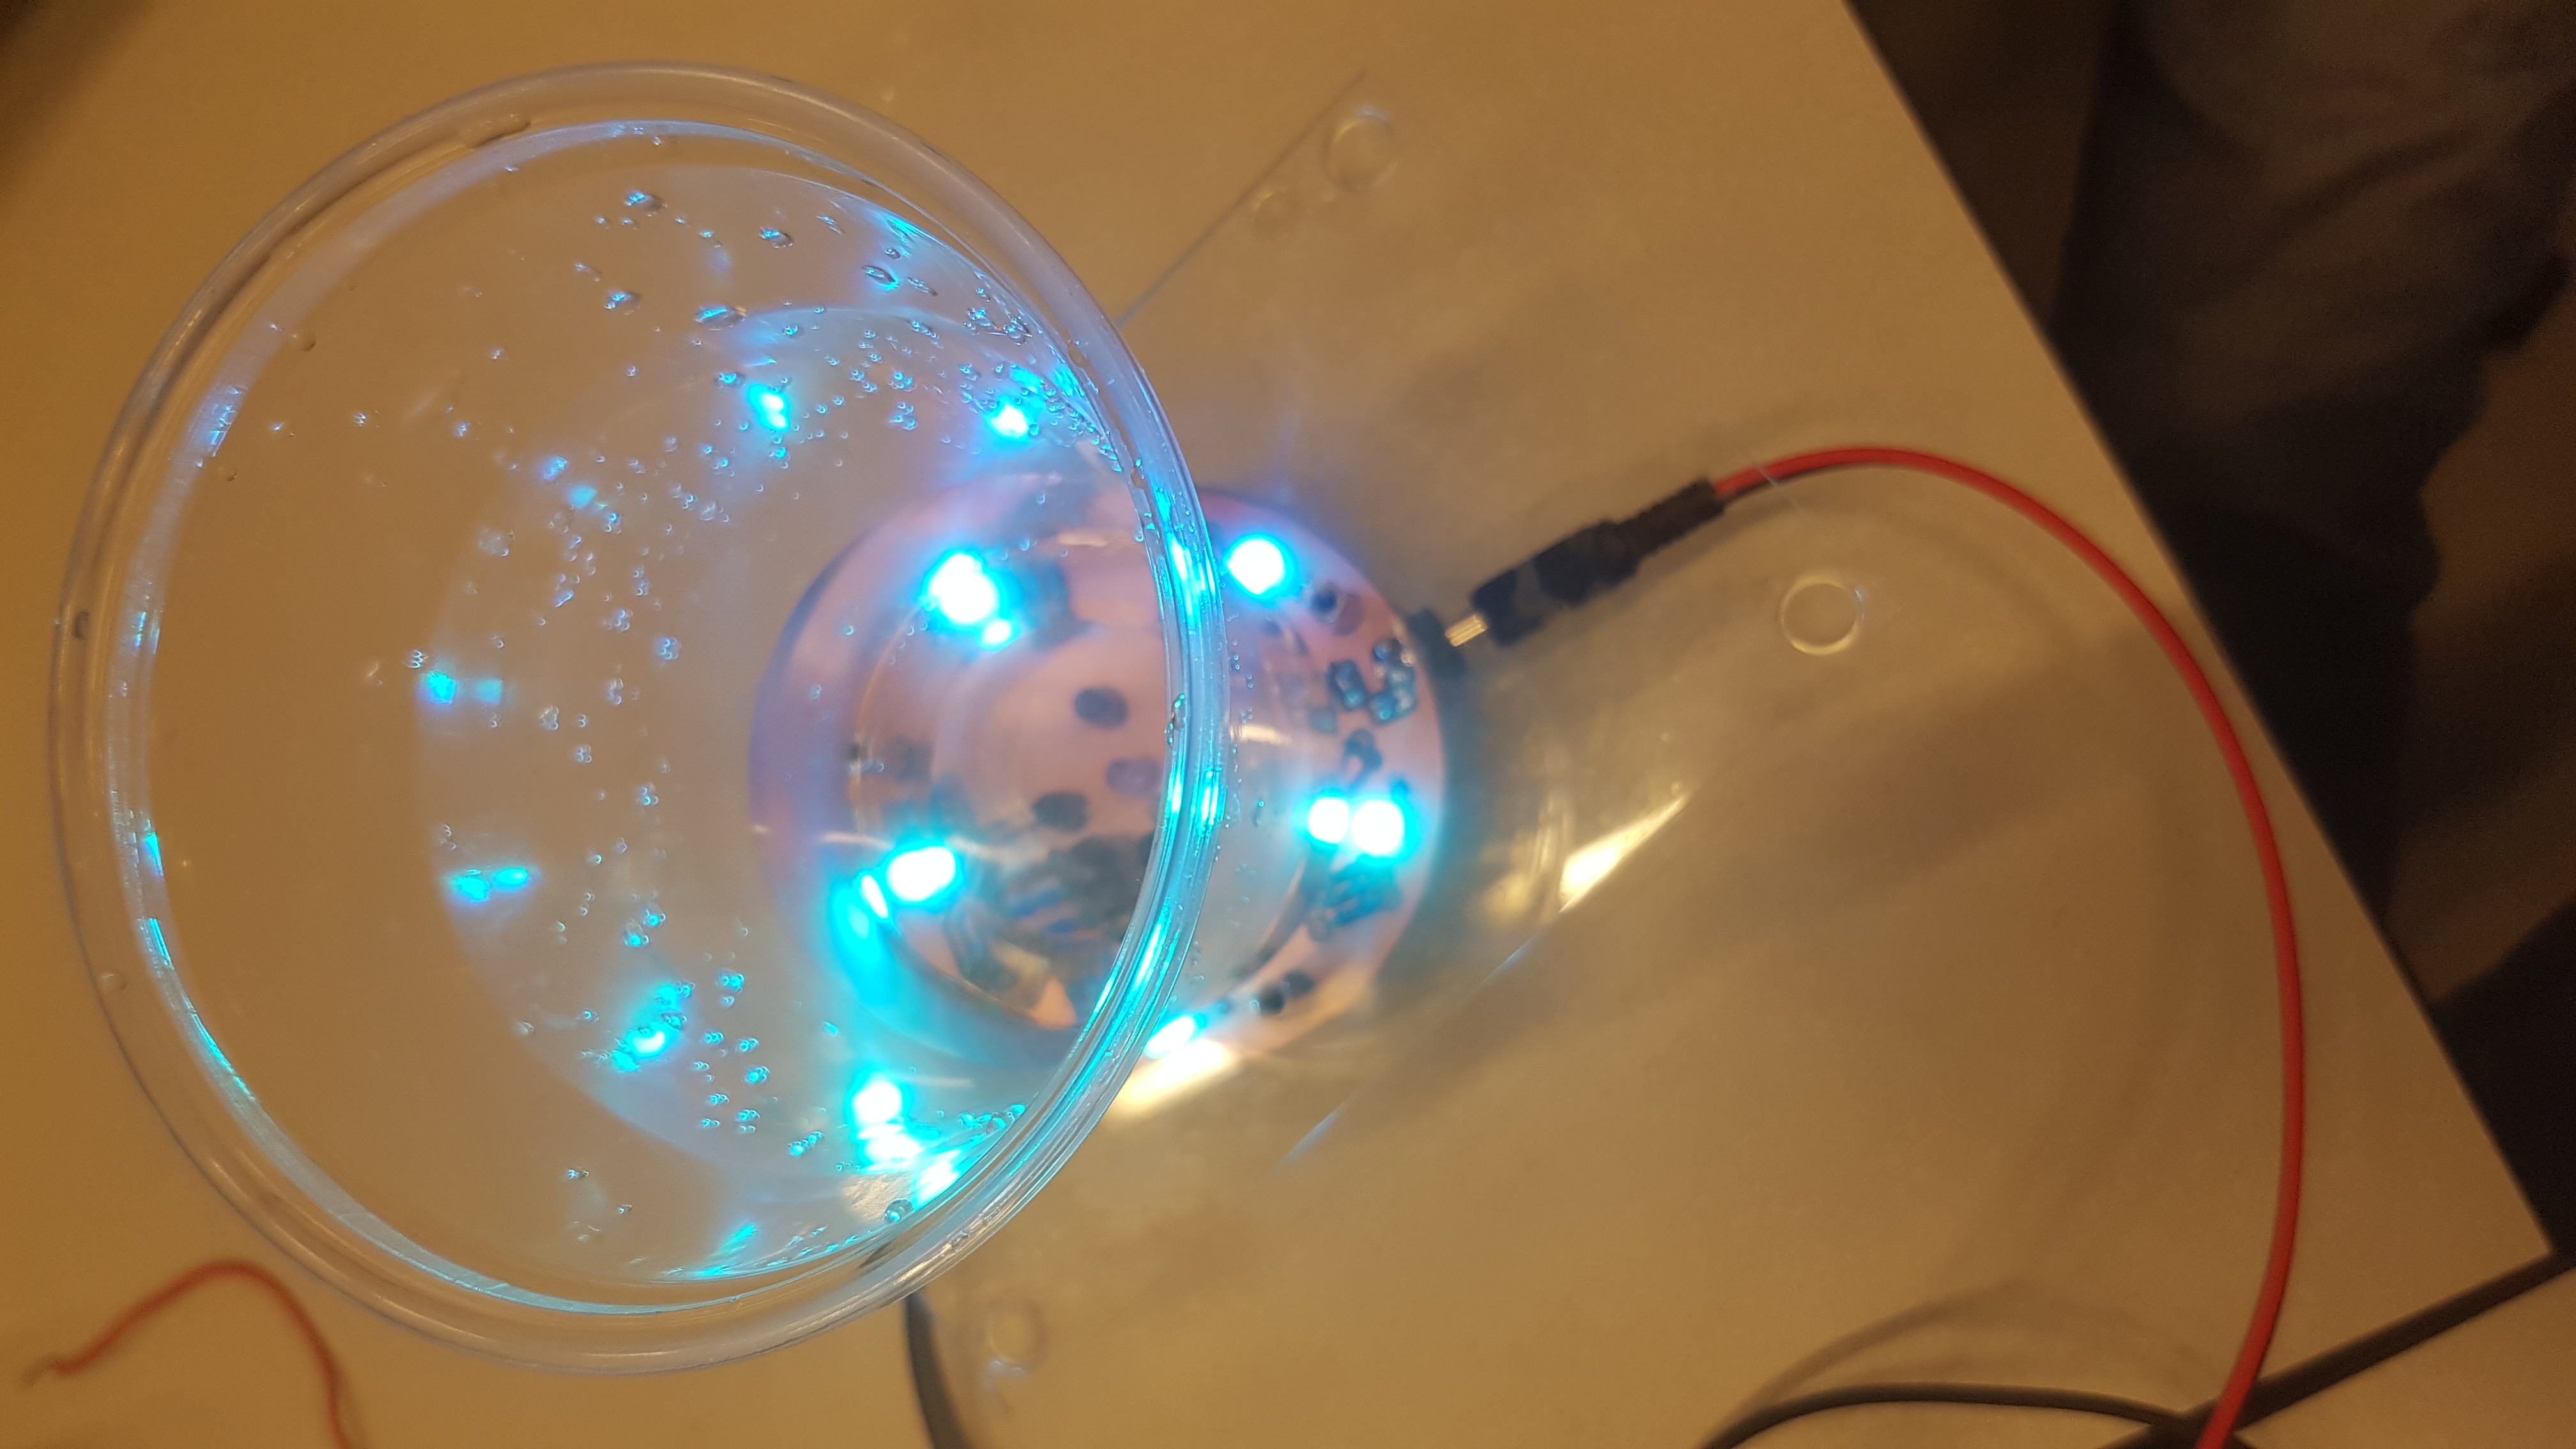
\includegraphics[width=\textwidth]{Integrationstest/Integrationstest_PlayerSide/graphics/CupSensorInt/PLAYING_my_col.jpg}
    \caption{PSoC playerside ved state PLAYING med kop}
    \label{fig:int_playerside_playing_my}
\end{figure}

Der kastes så en bold i koppen for at symbolisere at koppen er ramt. Hvilket giver følgende figur \ref{fig:int_playerside_playing_ball}
\begin{figure}[H]
    \centering
    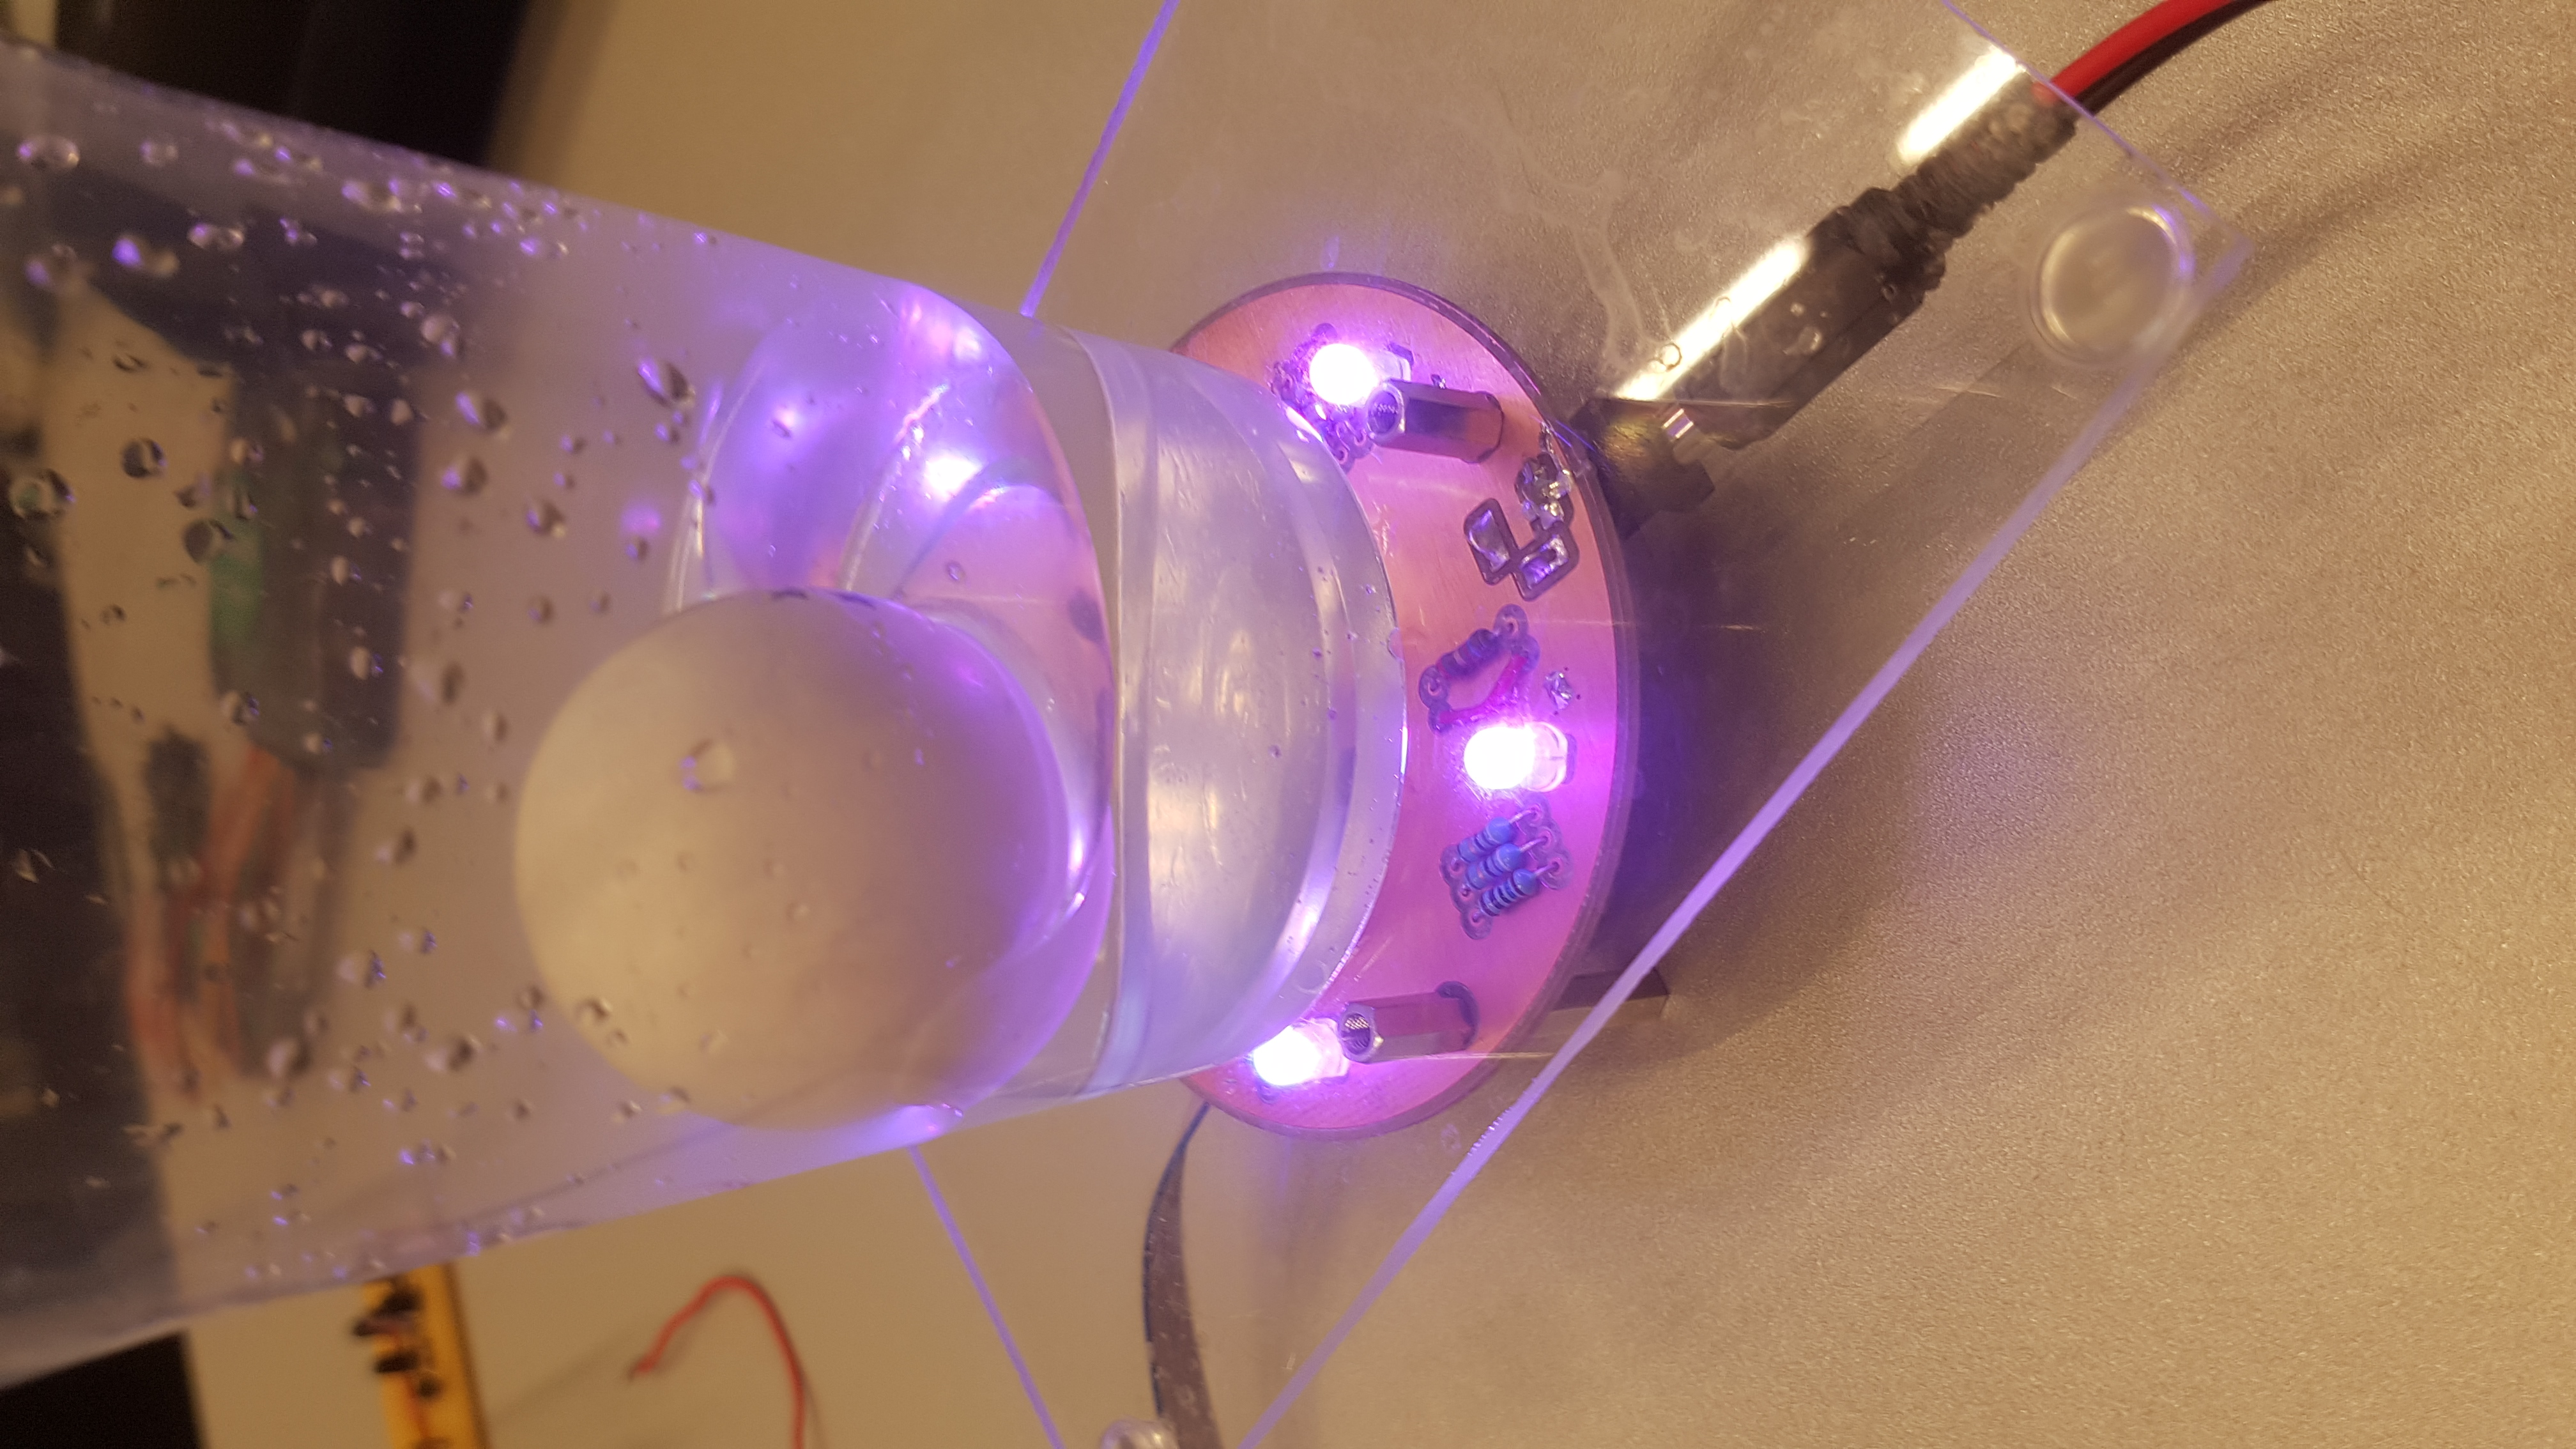
\includegraphics[width=\textwidth]{Integrationstest/Integrationstest_PlayerSide/graphics/CupSensorInt/PLAYING_blink.jpg}
    \caption{PSoC playerside ved state PLAYING med bold i kop}
    \label{fig:int_playerside_playing_ball}
\end{figure}

Når states så skifter til \textit{Won}, så kan dette testes ved at have en kop på kopholder og tvinge den til at skifte til state \textit{Won}. Dette ses i figur \ref{fig:int_playerside_won}. Her er det værd at pointere at det blev testet med at koppen blev taget af, for at sikre farven ikke skiftede.
\begin{figure}[H]
    \centering
    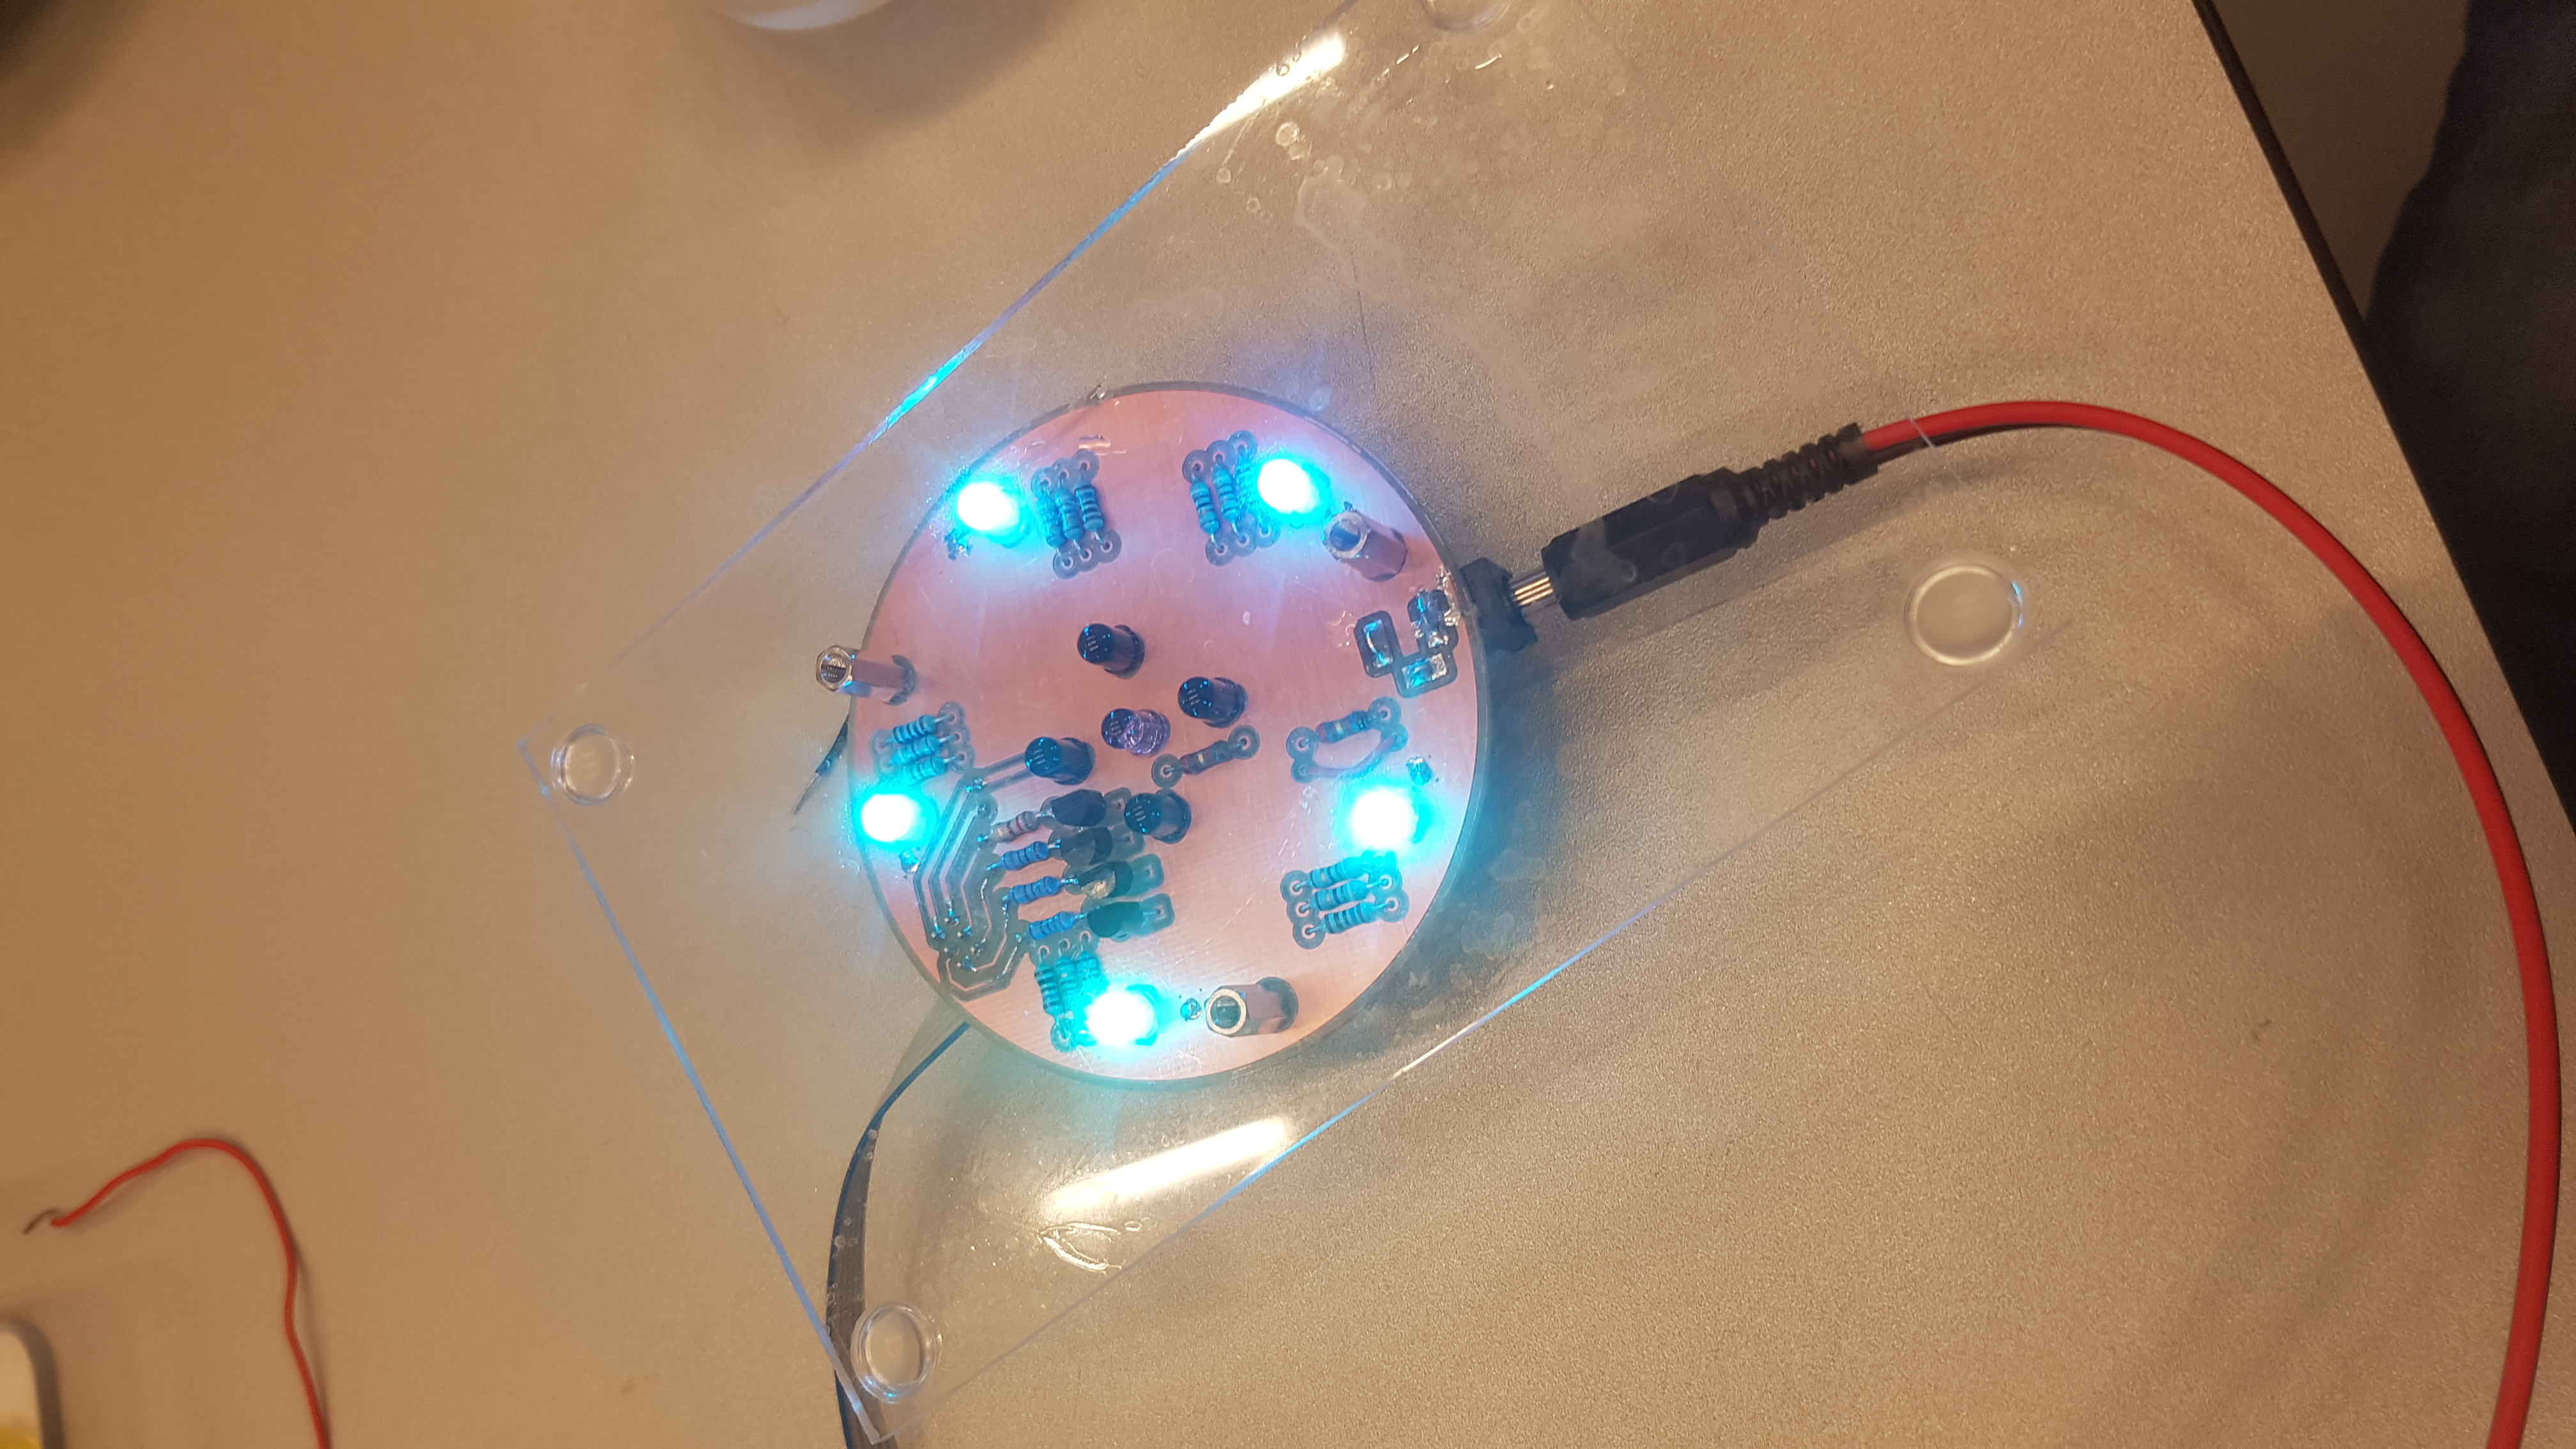
\includegraphics[width=\textwidth]{Integrationstest/Integrationstest_PlayerSide/graphics/CupSensorInt/WON.jpg}
    \caption{PSoC playerside ved state WON}
    \label{fig:int_playerside_won}
\end{figure}

Der skal også skiftes state til \textit{Lost}. Der testes på samme måde som \textit{won}. Dette ses i figur \ref{fig:int_playerside_loss}.
\begin{figure}[H]
    \centering
    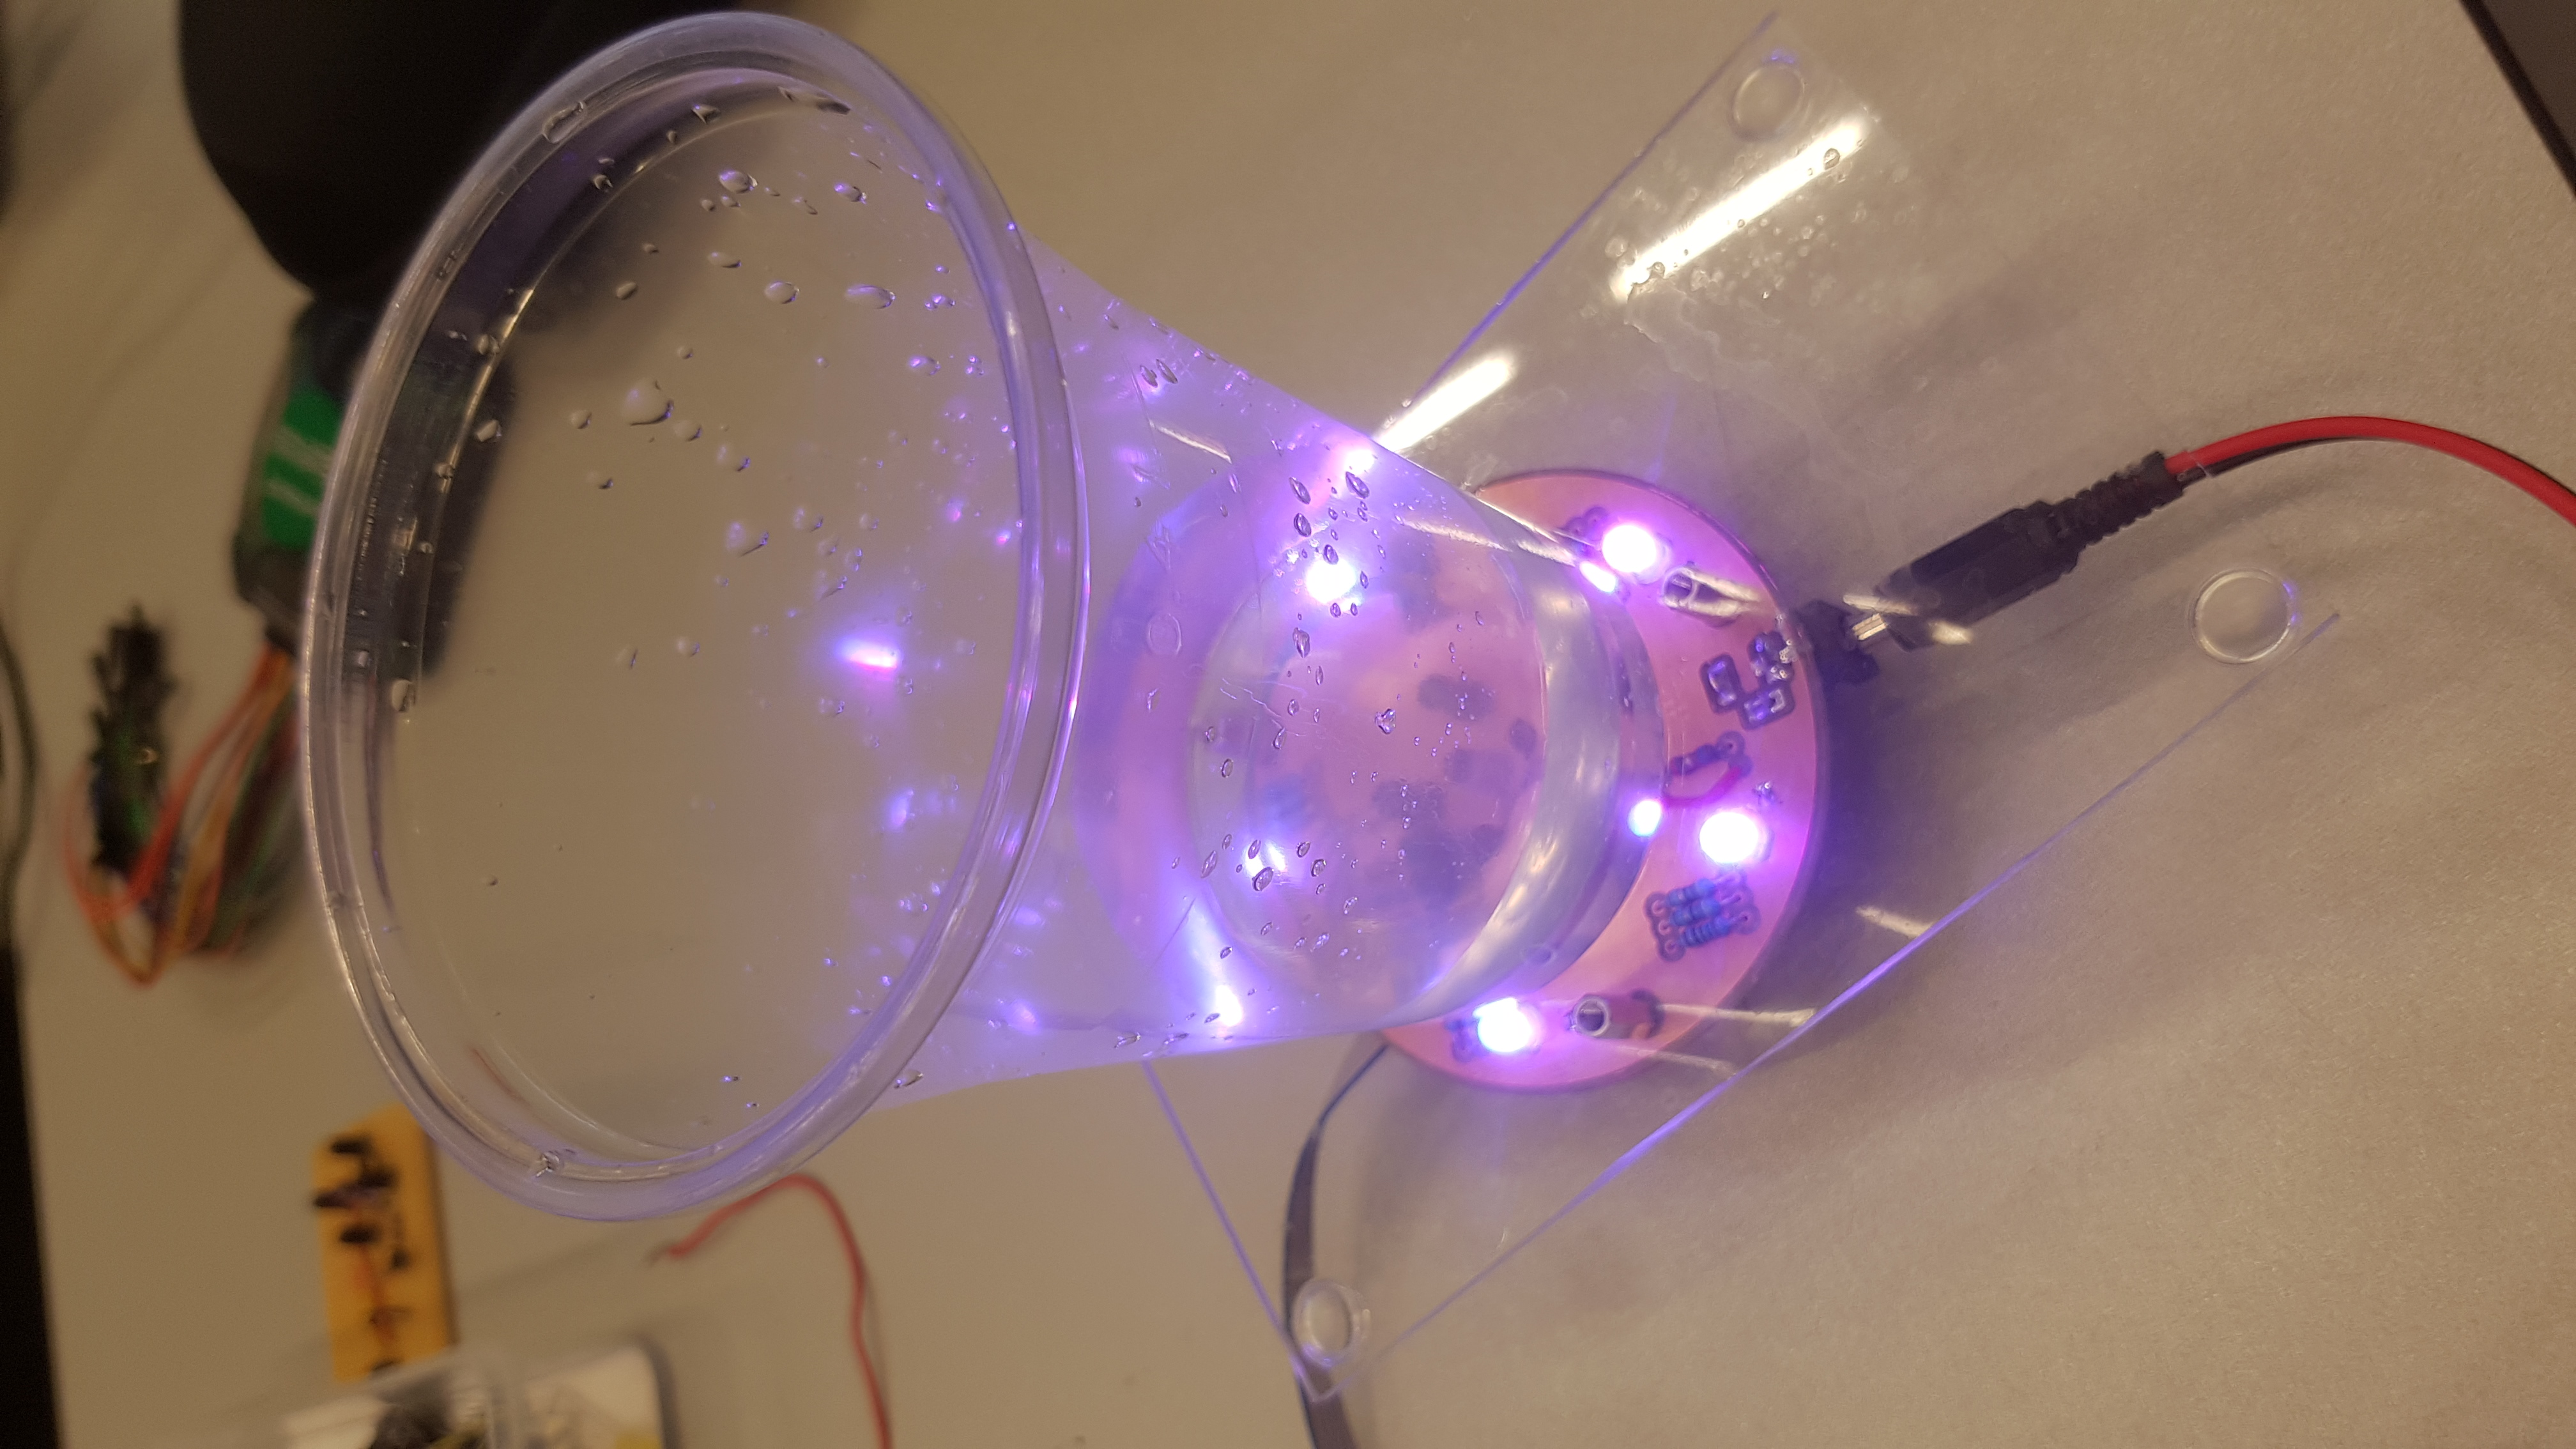
\includegraphics[width=\textwidth]{Integrationstest/Integrationstest_PlayerSide/graphics/CupSensorInt/LOST.jpg}
    \caption{PSoC playerside ved state LOST}
    \label{fig:int_playerside_loss}
\end{figure}


\subsection{Integrationstest med RPi\_IF}
Der skulle også testes integration i forhold til om  data der følger protokollen blev sendt fra PSoC-playerside til RPi på de rigtige tidspunkter. Dette modul var i princippet allerede testet med GameController, men det skulle verificeres at det stadig virker.

\subsubsection{Testopstilling}
Denne del af integrationen blev testet med samme opstilling som tidligere beskrevet, hvor den eneste forskel var at bruge AnalogDiscovery til at læse fra I2C på PSoC.

\subsubsection{Testudførelse}
Testene blev foretaget ved at tjekke om det rigtige data blev sendt i forhold til om en kop blev flyttet til kopholderen, fra kopholderen eller der blev ramt en bold i koppen. Dette blev som sagt målt med AnalogDiscovery2 ved at bruge Protocol funktionen i WaveForms.

\subsubsection{Resultater}
Da modultesten for RPI\_IF allerede har testet protokollen, og der ingen ændringer var i forhold til denne, så beskrives den ikke yderligere end at konstatere at resultaterne var de samme.


\subsection{Refleksion}
Af de foregående resultat afsnit ses det, at systemet fungere i forbindelse med hvilket lys, der bliver vist, i forbindelse med den detektering af events  ved placering af, fjernelse af og bold i kop, samt systemets navigation mellem states.

I integrationstesten har der været flere små fejl, der har forstyrret integreringen mellem de forskellige komponenter. Startes der med den største fejl, så blev den tydelig da der blev læst CupStatus via I2C kommunikation fra PSoC. Der skete en fejl, hvor at der blev modtaget forkert data i forhold til det forventede. Denne fejl blev isoleret til, at da der blev kombineret mange forskellige interrupts, og de havde samme prioritet, så skabte det en fejl, hvor I2C blev interruptet midt i sit eget. Denne fejl blev umiddelbart løst ved at ændre prioriteterne af de forskellige interrupts til noget fornuftigt. Det dumme ved dette er, at vi flere gange inden har haft prioriteterne oppe og diskutere, men dette blev bare glemt under selve intergreringen. De valgte prioriteter ses i figur \ref{fig:int_interrupt_priorities}, hvor lavt tal er høj prioritet.
\begin{figure}[H]
    \centering
    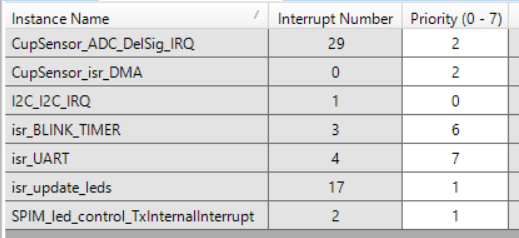
\includegraphics[width=\textwidth]{Integrationstest/Integrationstest_PlayerSide/graphics/CupSensorInt/Interrupts_prio.png}
    \caption{De opdaterede prioriteter for interrupts}
    \label{fig:int_interrupt_priorities}
\end{figure}

Der var også forskellige små fejl i forskelligt logik i gamecontrolleren, som blev tydeliggjort af integrationstesten og fikset herefter.

Derudover var der en fejl i integreringen af CupLight, da der kun blev lavet en test for en kopholder, hvilket ikke blev taget ordentligt hånd om. Efter at opdatering af en parameter var dette problem også løst.

Den største fejlkilde ved denne intergreringstest var, at det ikke var muligt at få produceret nok \textit{CupHolders} til at teste hele PlayersideSystemet. Der er dog tiltro til rubustheden af det udviklede system i forbindelse med de forskellige samlede moduler, men der skal laves en genopfyldende test med samtlige kopholder for at sikre integreringen. 

\subsection{Konklusion}
Det kan altså konkluderes at der er blevet lavet et samlet integreret modul, der virker for PSoC PlayerSide, hvor det er muligt at imitere hele spil forløbet i forbindelse med et spil Beer Pong. Selvom testen ikke er helt fyldestgørende på grund af manglende CupHolders, giver det stadig et godt indblik i om systemet virker når det er fuldt samlet. Selve intergrationen af undermodulerne til et samlet modul har været forholdsvis smertefrit, da arkitekturen havde været god nok til, at få tingene til at passe sammen i forvejen. Derudover blev der heller ikke taget nogen design-valg, der havde for stor negativ indflydelse på de andre moduler. Det kunne f.eks. være generende støj, mellem hardware modulerne eller ting i software, der påvirkede andet software.

\end{document}